% created on 28/07/2020
% @author : ebazan
\part{Image Contours}

\chapter{Unsupervised Object Detection for UAV Autonomous Landing task}
The detection of a target for the UVA autonomous landing nowadays is a recurring subject in the industrial sector. Precisely, the idea of this project is inspired by the needs of the Internest company \cite{InternestWeb}. We show two algorithms developed for the landing target detection; the first, a continuation of the work developed during the traineeship period of a master student \cite{BaquedanoA.:ESIEE:2017} and the second, a more general approach that explores the principles of human perception.

\section{Image Contour Detection Methods}
This first approach seeks to solve the task straightforwardly using highly studied techniques. The algorithm is based on finding the contours of a binary image generated by the thresholding method proposed by Otsu \cite{Otsu:SMC:1979}. It use heuristically the hierarchy of the found contours to detect the landing target because the landing target is formed by concentric circles (see appendix \ref{ch:target_description}). 

The idea was tested, however, same as some works of section \ref{sec:problems}, the algorithm works well only under certain circumstances. Diverse factors, such as noise, changes in lighting, contrast, size of the object w.r.t. the scene, complicate the operation of thresholding and consequently the contour detection. We classify the perturbations suffered by the landing targets in four groups: change in size w.r.t. the scene, presence of noise, presence of shadows and deformation due to perspective. Figure \ref{fig:tar_degradations} shows a the landing target affected by the aforementioned disturbances.

\begin{figure}[!ht]
    \centering
    \begin{subfigure}[b]{0.3\textwidth}
        \frame{
\includegraphics[width=\textwidth]{tar_noise}}
        \caption{}
        \label{fig:deg_noise}
    \end{subfigure}
        ~ %add desired spacing between images, e. g. ~, \quad, \qquad, \hfill etc. 
      %(or a blank line to force the subfigure onto a new line)
    \begin{subfigure}[b]{0.3\textwidth}
        \frame{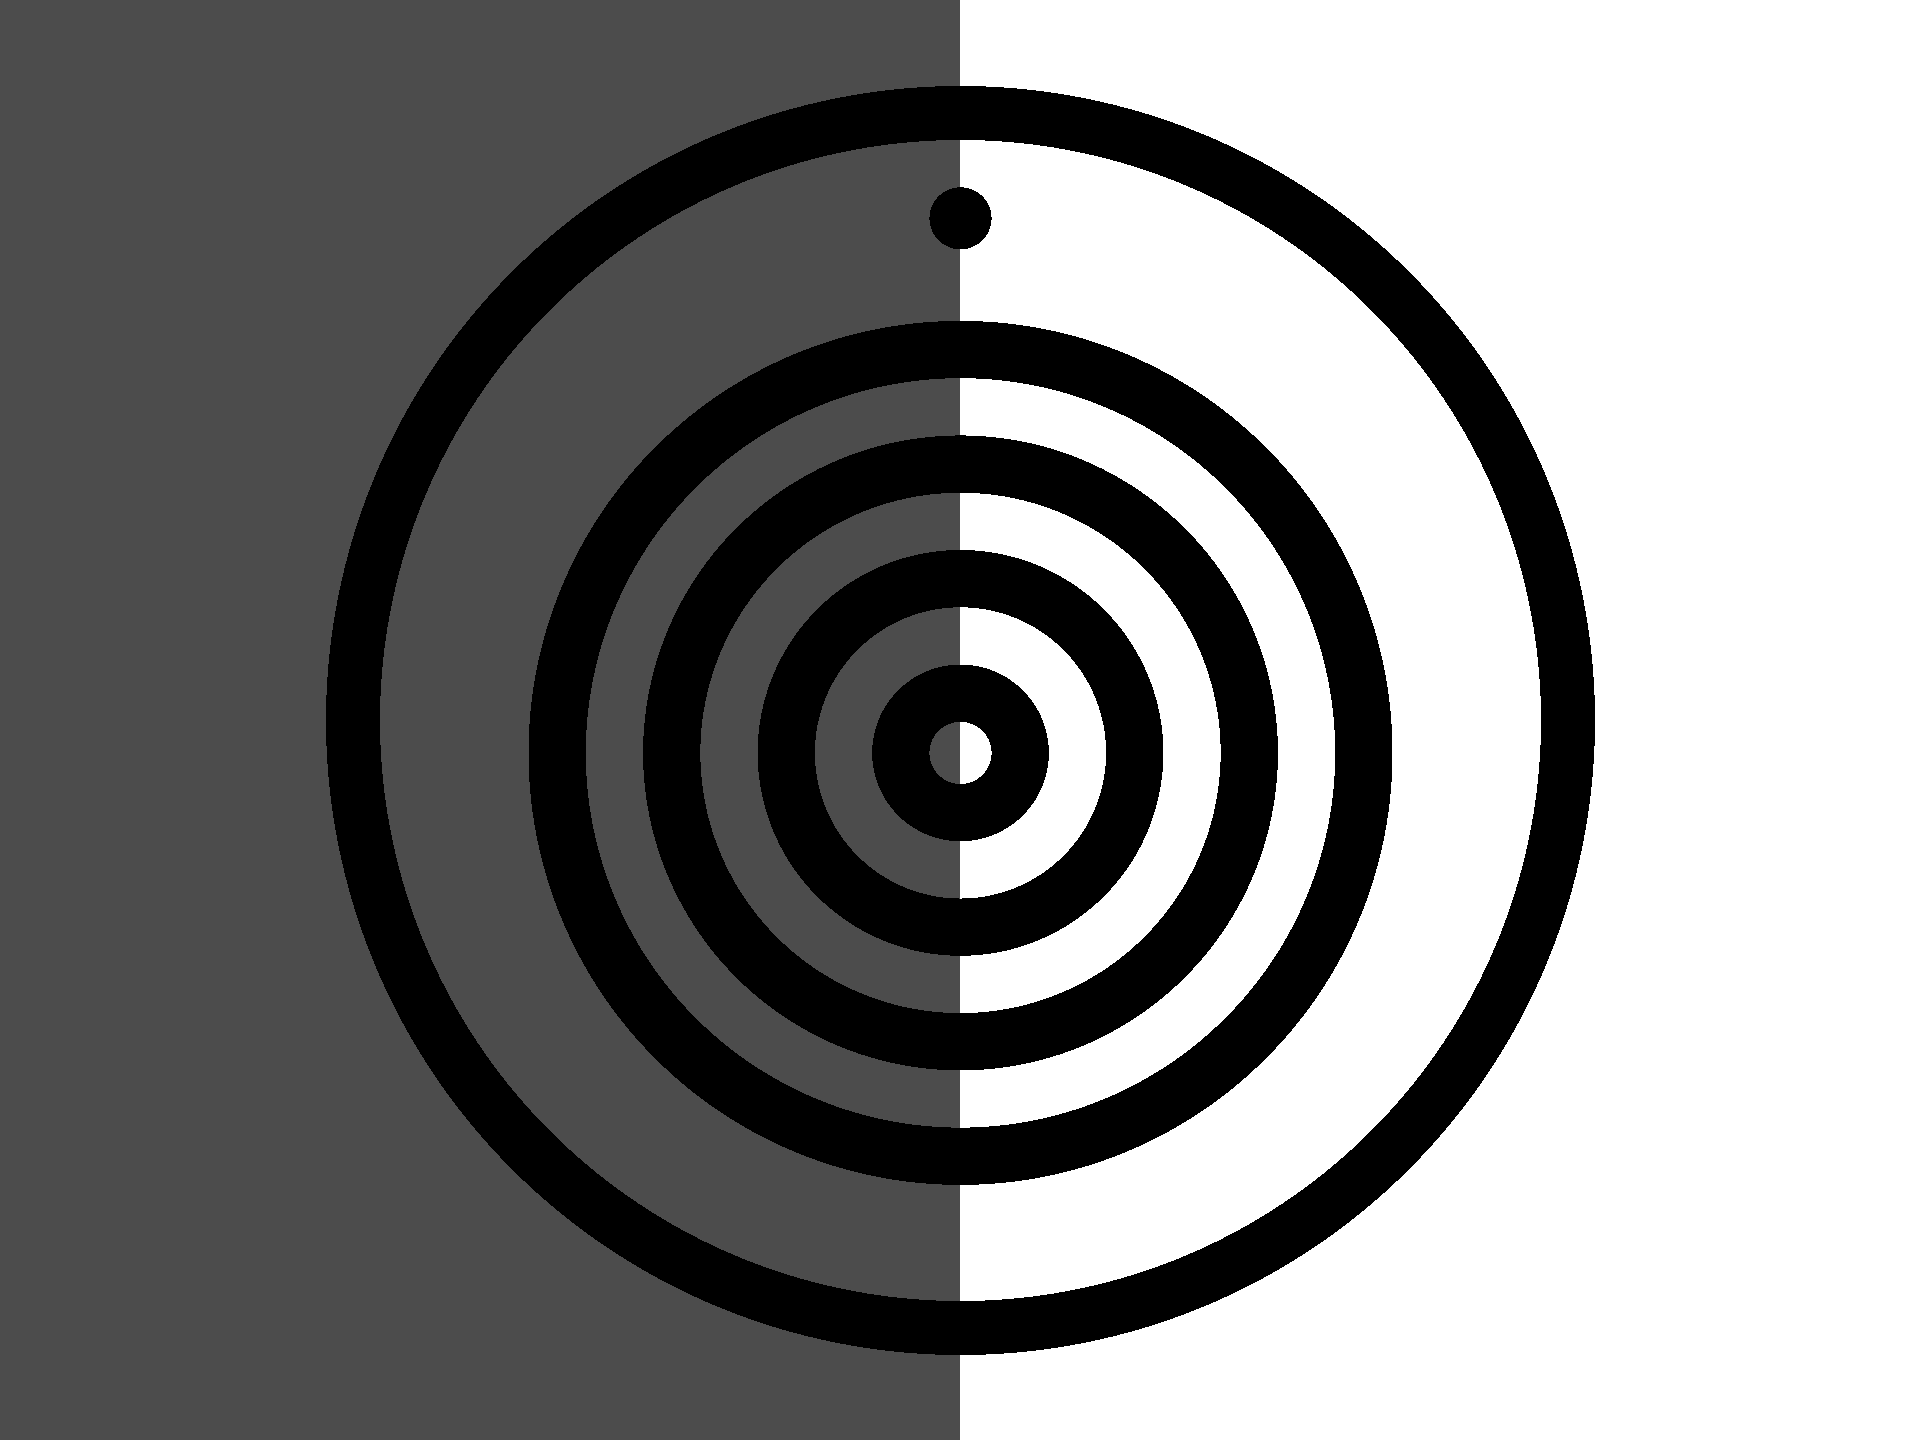
\includegraphics[width=\textwidth]{tar_shadow}}
        \caption{}
        \label{fig:deg_shadow}
    \end{subfigure}\\
        ~ %add desired spacing between images, e. g. ~, \quad, \qquad, \hfill etc. 
      %(or a blank line to force the subfigure onto a new line)
    \begin{subfigure}[b]{0.3\textwidth}
        \frame{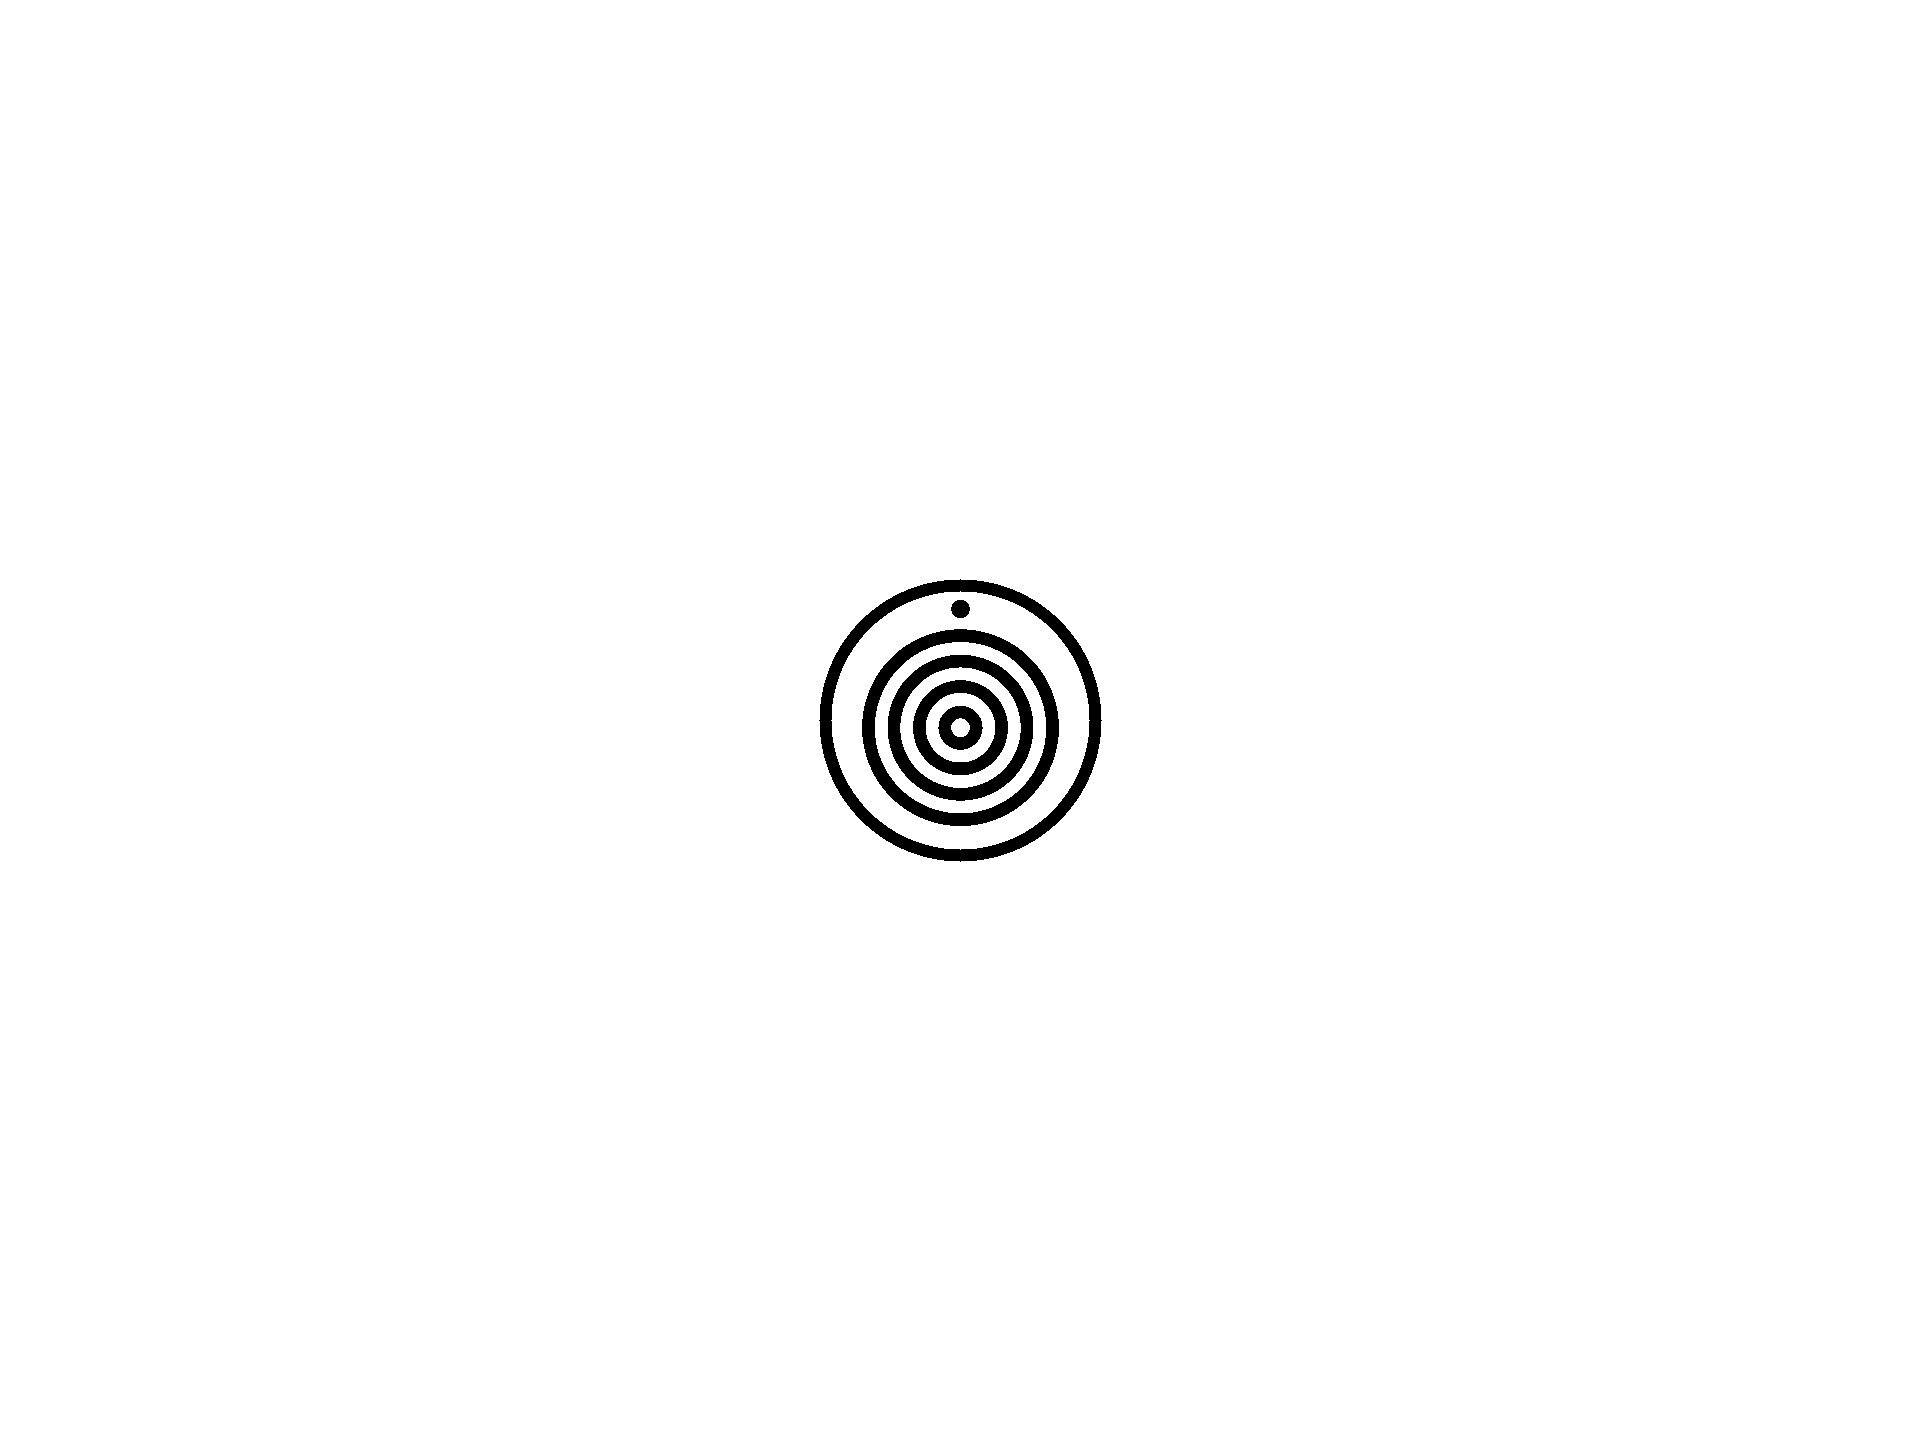
\includegraphics[width=\textwidth]{tar_resolution}}
        \caption{}
        \label{fig:deg_resolution}
    \end{subfigure}
        ~ %add desired spacing between images, e. g. ~, \quad, \qquad, \hfill etc. 
      %(or a blank line to force the subfigure onto a new line)
    \begin{subfigure}[b]{0.3\textwidth}
        \frame{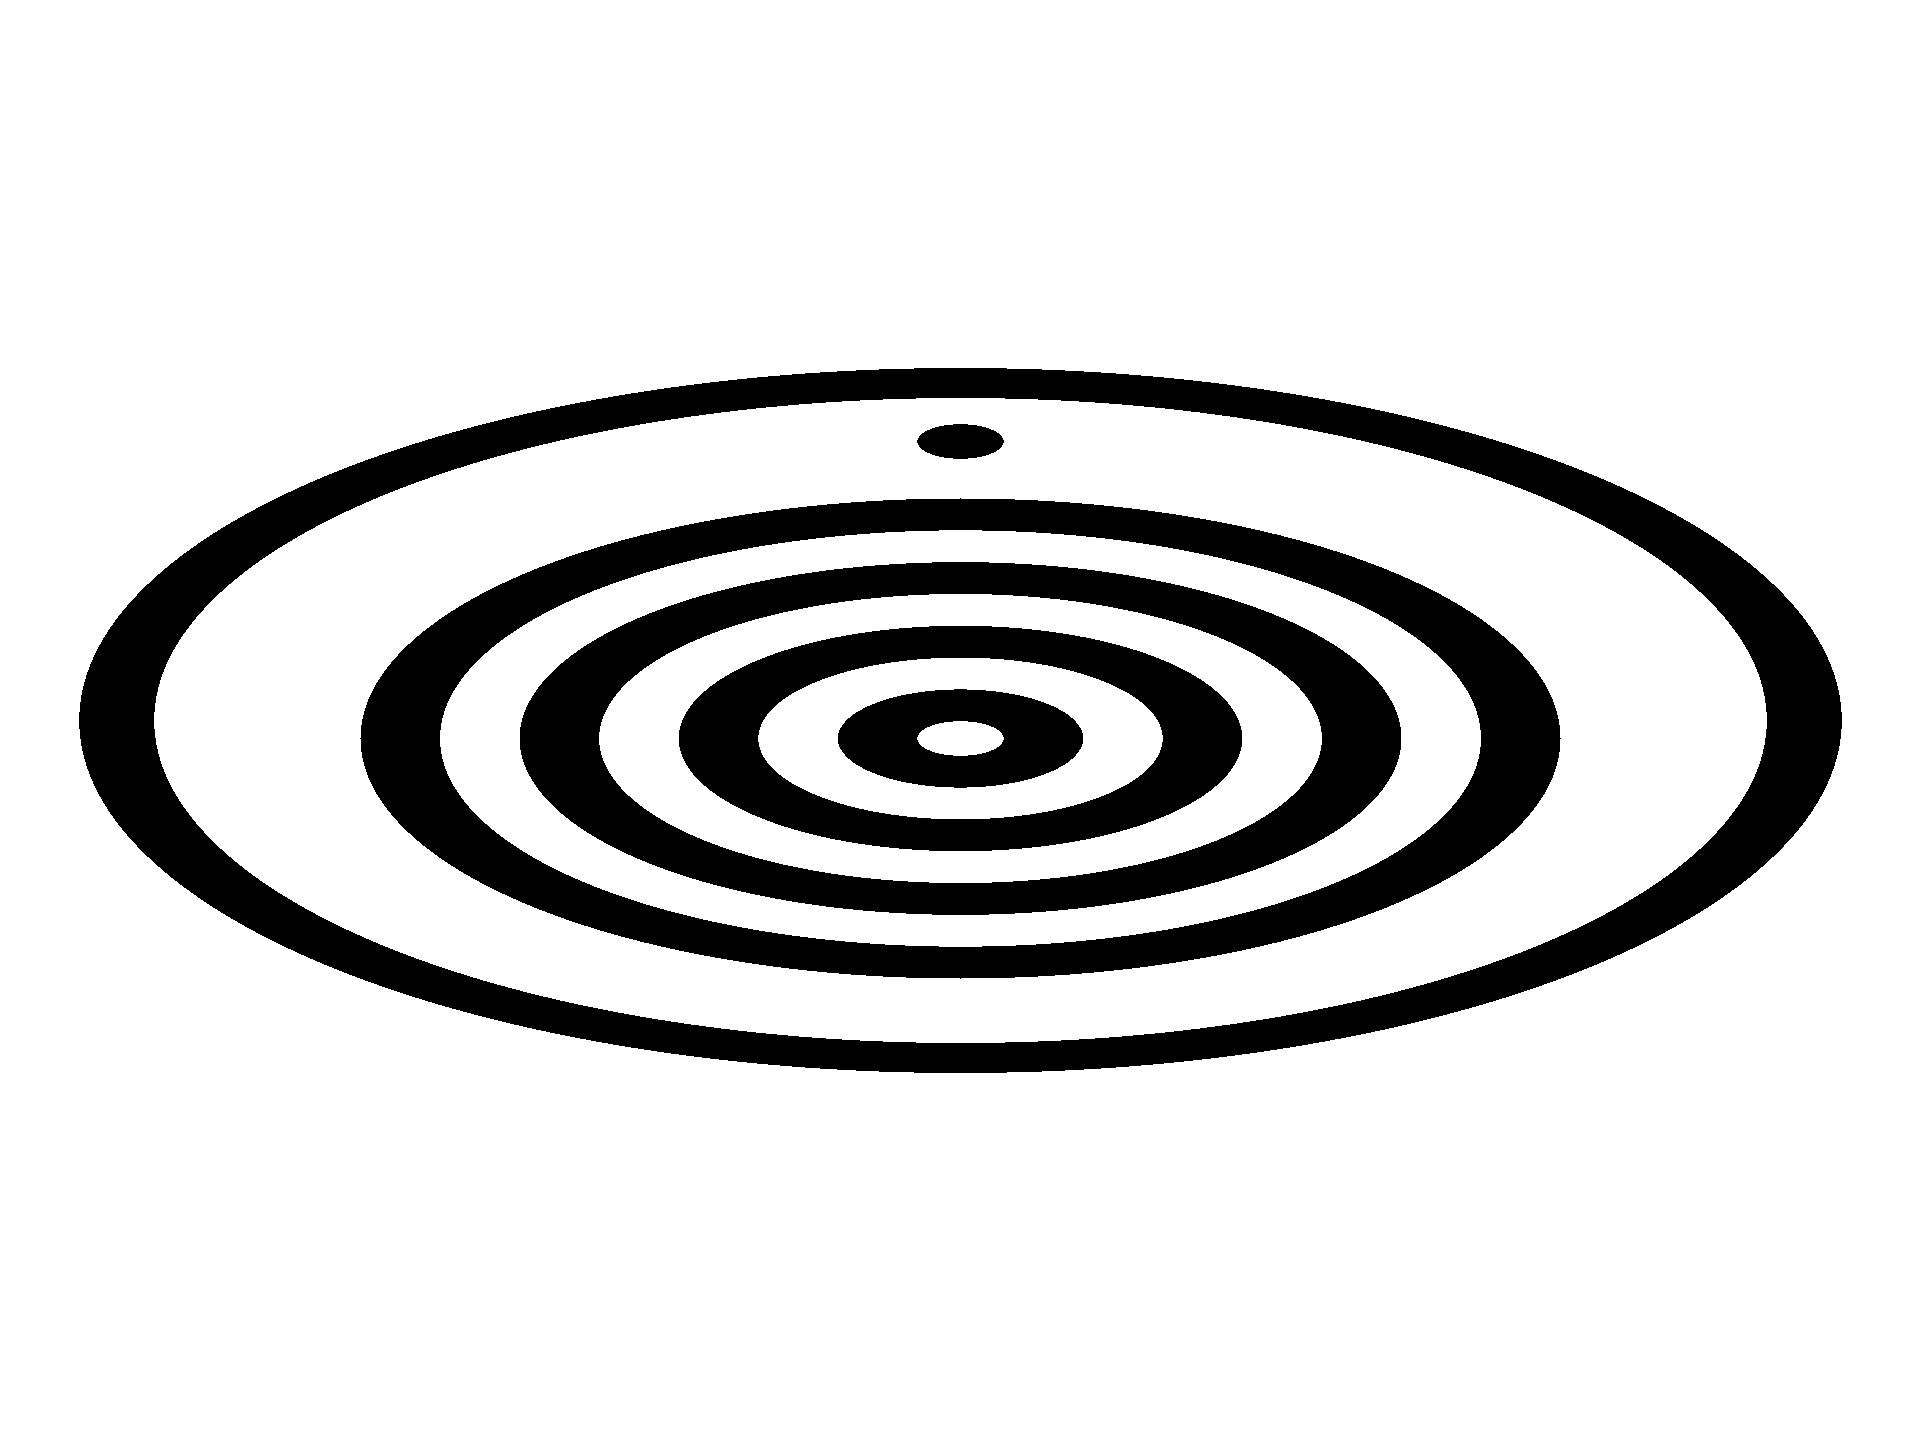
\includegraphics[width=\textwidth]{tar_deformation}}
        \caption{}
        \label{fig:deg_deformation}
    \end{subfigure}
    \caption{ Landing target degradations: \textbf{(a)} Noise, \textbf{(b)} Shadow, \textbf{(c)} Change of size and \textbf{(d)} Perspectice deformation}\label{fig:tar_degradations}
\end{figure}

\begin{figure}[htbp]
\centering
\begin{subfigure}[t]{\dimexpr0.15\textwidth+20pt\relax}
    \makebox[20pt]{\raisebox{30pt}{\rotatebox[origin=c]{90}{Input}}}%Input (zoom)
    \frame{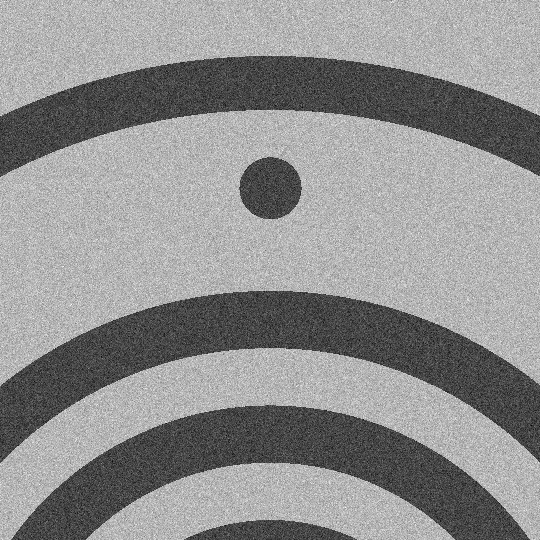
\includegraphics[width=\dimexpr\linewidth-20pt\relax]
    {tar_zoom_noise}}
    \makebox[20pt]{\raisebox{30pt}{\rotatebox[origin=c]{90}{Otsu}}}%
    \frame{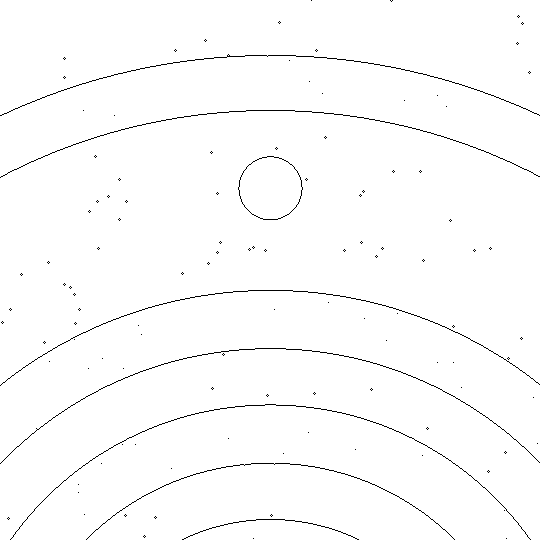
\includegraphics[width=\dimexpr\linewidth-20pt\relax]
    {Otsu_cont_noise}}
    \makebox[20pt]{\raisebox{30pt}{\rotatebox[origin=c]{90}{Riddler}}}%
    \frame{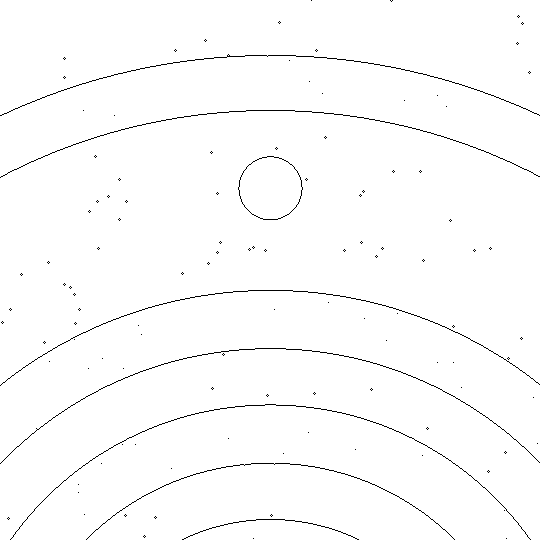
\includegraphics[width=\dimexpr\linewidth-20pt\relax]
    {Riddler_cont_noise}}
    \makebox[20pt]{\raisebox{30pt}{\rotatebox[origin=c]{90}{Yen}}}%
    \frame{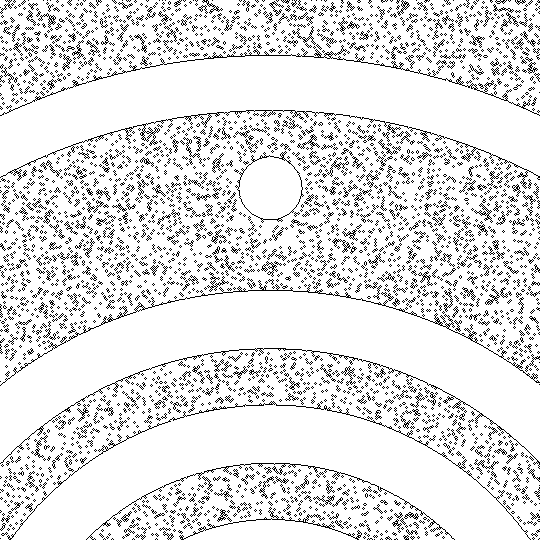
\includegraphics[width=\dimexpr\linewidth-20pt\relax]
    {Yen_cont_noise}}
    \makebox[20pt]{\raisebox{30pt}{\rotatebox[origin=c]{90}{Li}}}%
    \frame{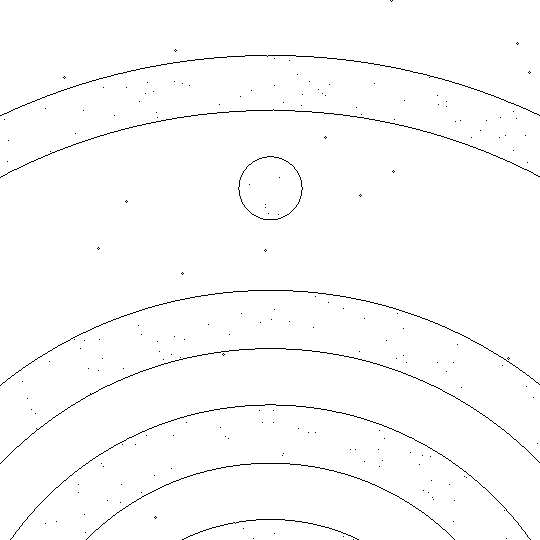
\includegraphics[width=\dimexpr\linewidth-20pt\relax]
    {Li_cont_noise}}
    \makebox[20pt]{\raisebox{30pt}{\rotatebox[origin=c]{90}{Niblack}}}%
    \frame{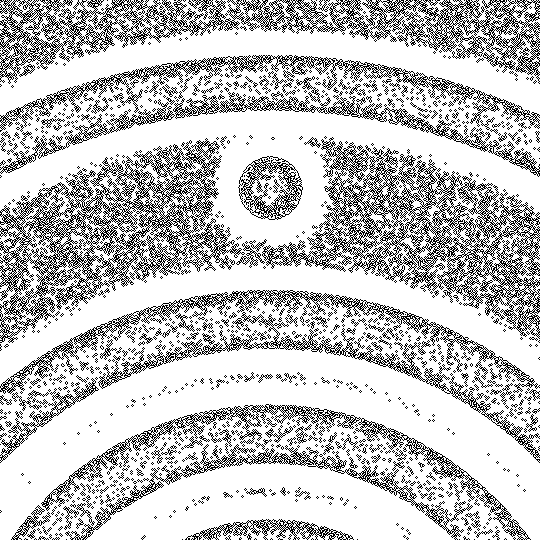
\includegraphics[width=\dimexpr\linewidth-20pt\relax]
    {Niblack_cont_noise}}
    \makebox[20pt]{\raisebox{30pt}{\rotatebox[origin=c]{90}{Sauvola}}}%
    \frame{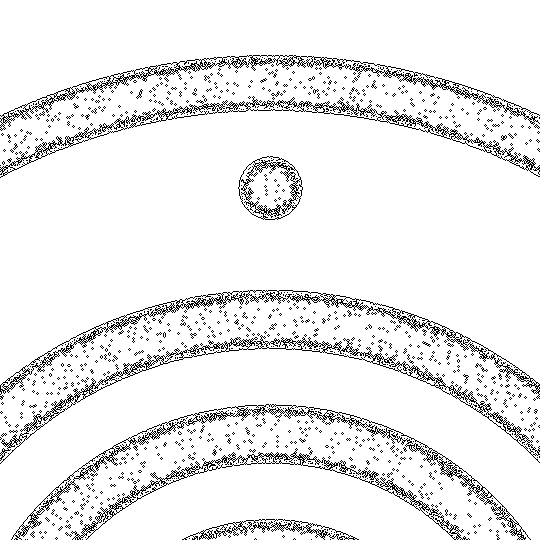
\includegraphics[width=\dimexpr\linewidth-20pt\relax]
    {Sauvola_cont_noise}}
    \makebox[20pt]{\raisebox{30pt}{\rotatebox[origin=c]{90}{Bradley}}}%
    \frame{
\includegraphics[width=\dimexpr\linewidth-20pt\relax]
    {Bradley_cont_noise}}
    \makebox[20pt]{\raisebox{30pt}{\rotatebox[origin=c]{90}{Gauss}}}%
    \frame{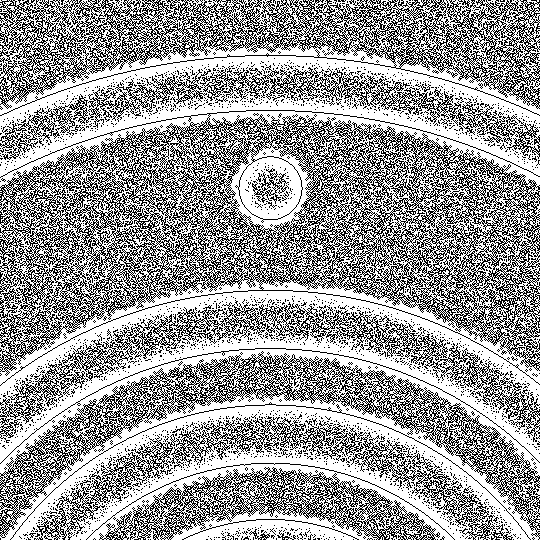
\includegraphics[width=\dimexpr\linewidth-20pt\relax]
    {Gauss_cont_noise}}
    \makebox[20pt]{\raisebox{30pt}{\rotatebox[origin=c]{90}{Mean}}}%
    \frame{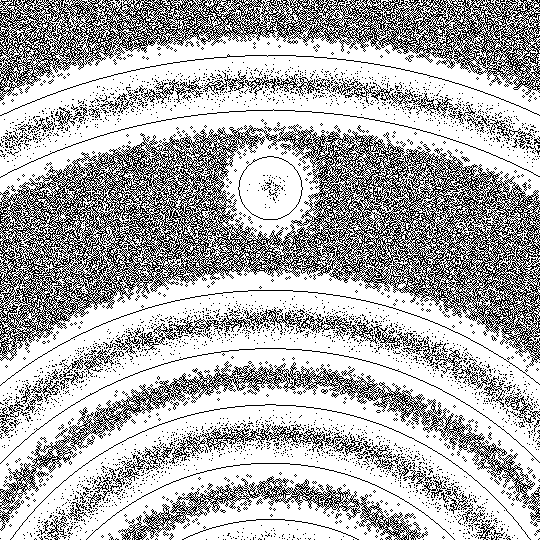
\includegraphics[width=\dimexpr\linewidth-20pt\relax]
    {Mean_cont_noise}}
    \caption{} 
\end{subfigure}\qquad
\begin{subfigure}[t]{0.15\textwidth}
    \frame{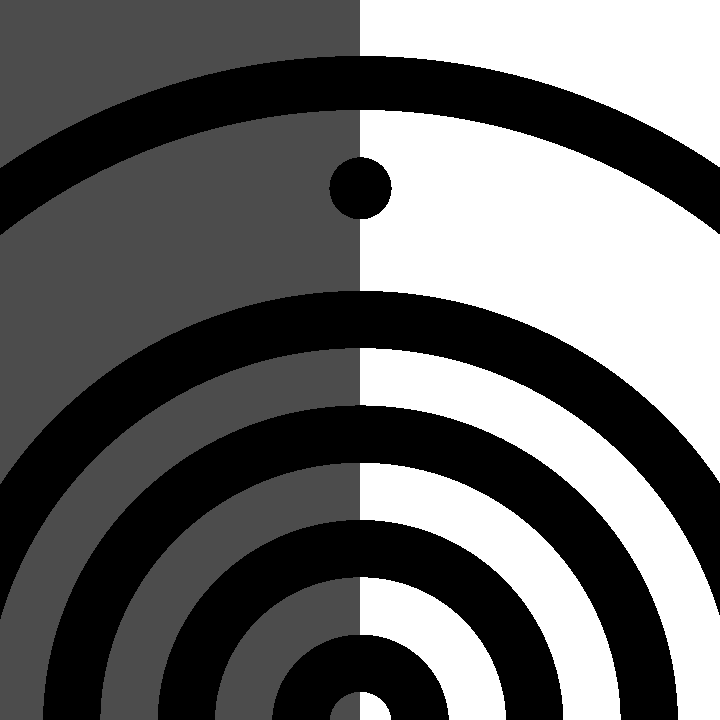
\includegraphics[width=\textwidth]
    {tar_zoom_shadow}}
    \frame{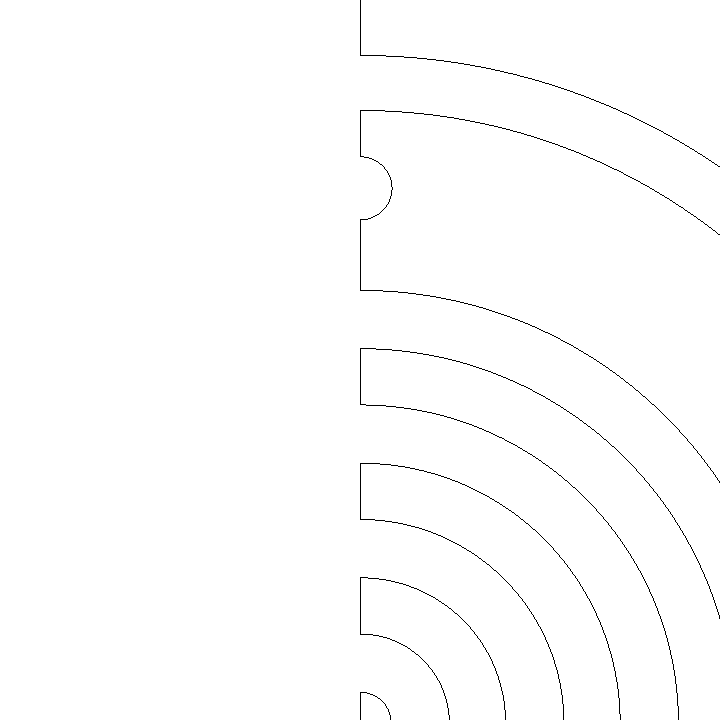
\includegraphics[width=\textwidth]
    {Otsu_cont_shadow}}
    \frame{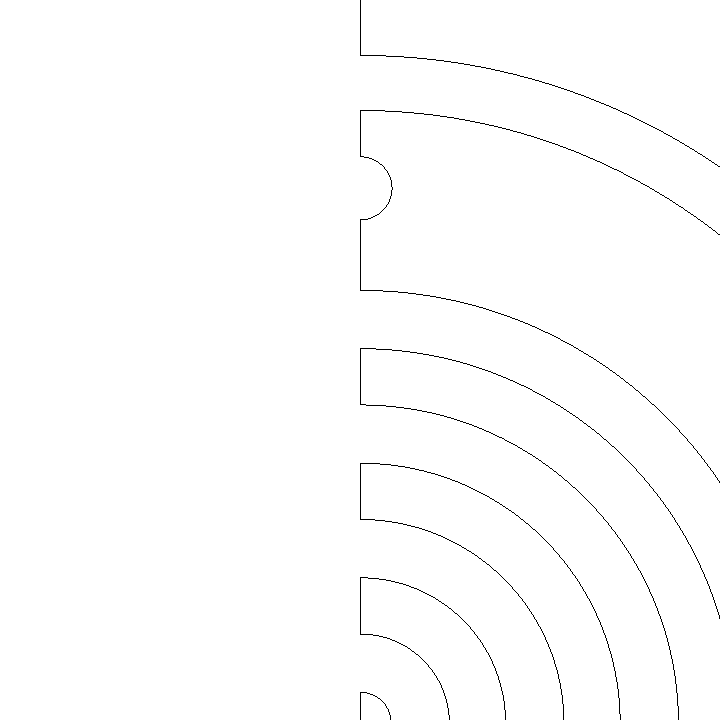
\includegraphics[width=\textwidth]
    {Riddler_cont_shadow}}
    \frame{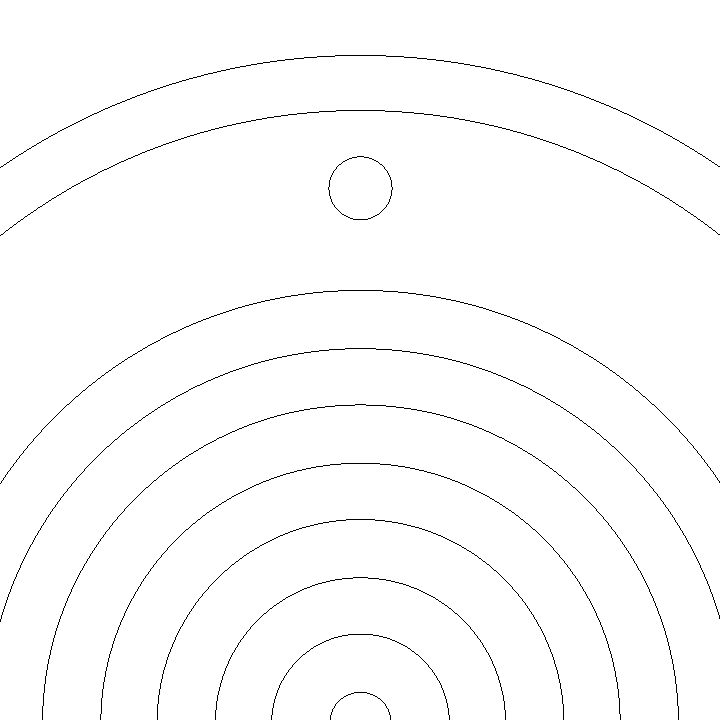
\includegraphics[width=\textwidth]
    {Yen_cont_shadow}}
    \frame{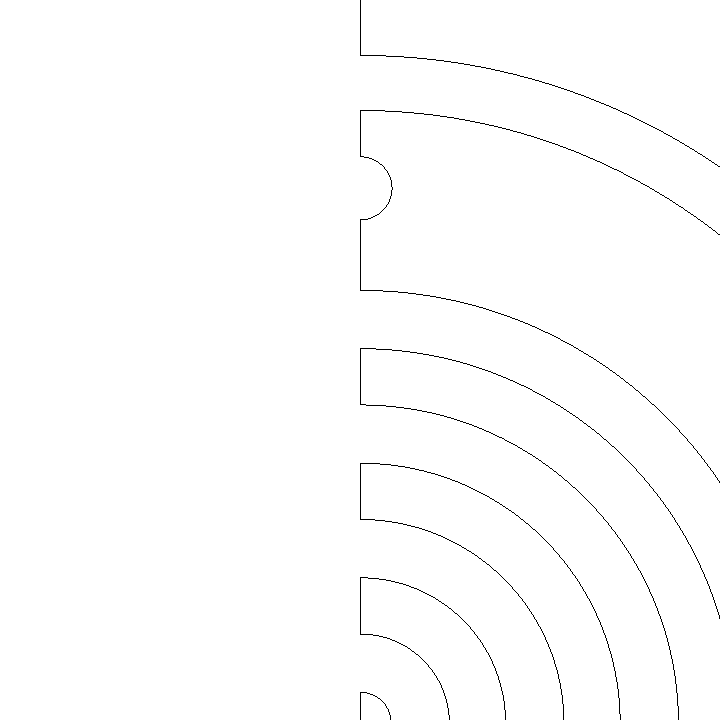
\includegraphics[width=\textwidth]
    {Li_cont_shadow}}
    \frame{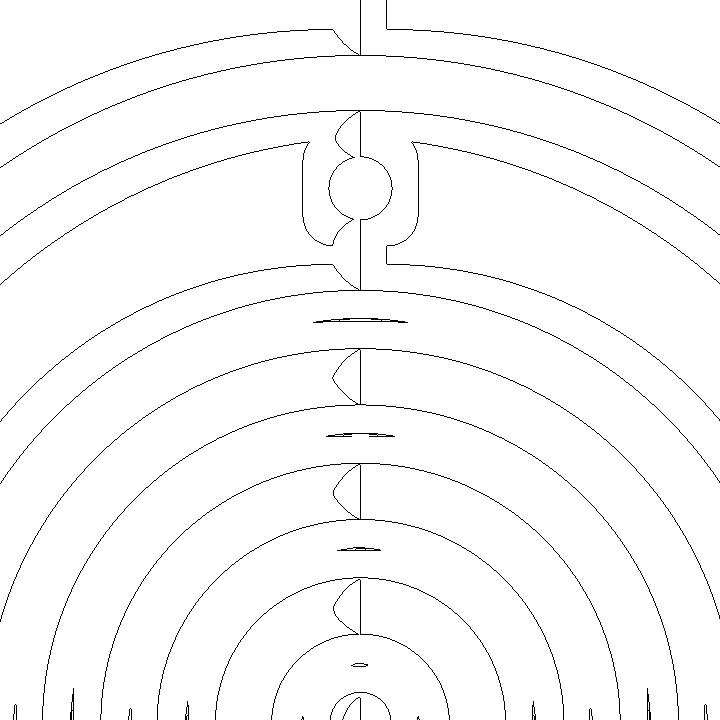
\includegraphics[width=\textwidth]
    {Niblack_cont_shadow}}
    \frame{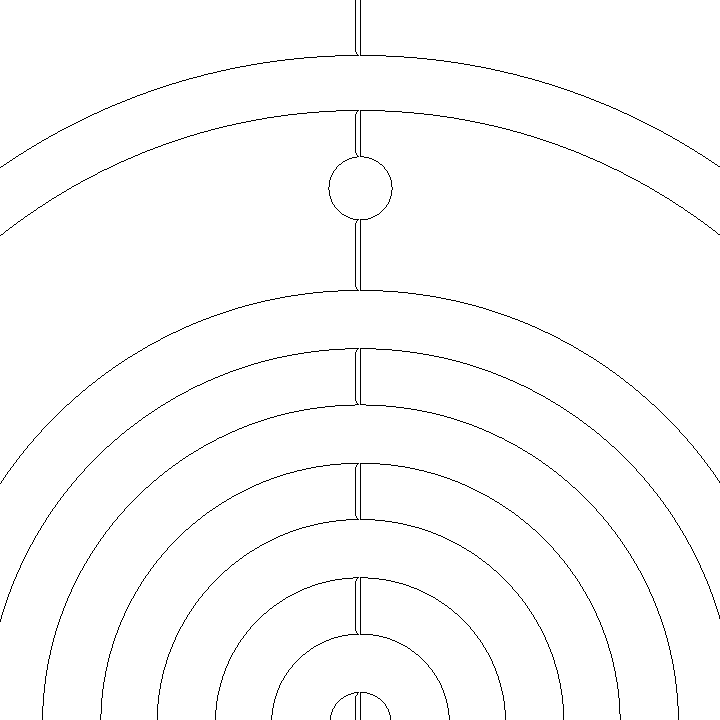
\includegraphics[width=\textwidth]
    {Sauvola_cont_shadow}}
    \frame{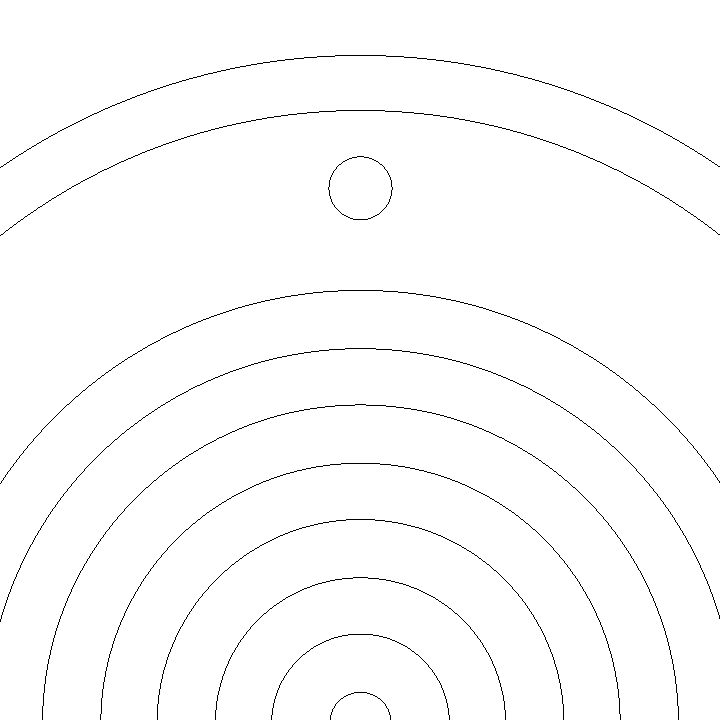
\includegraphics[width=\textwidth]
    {Bradley_cont_shadow}}
    \frame{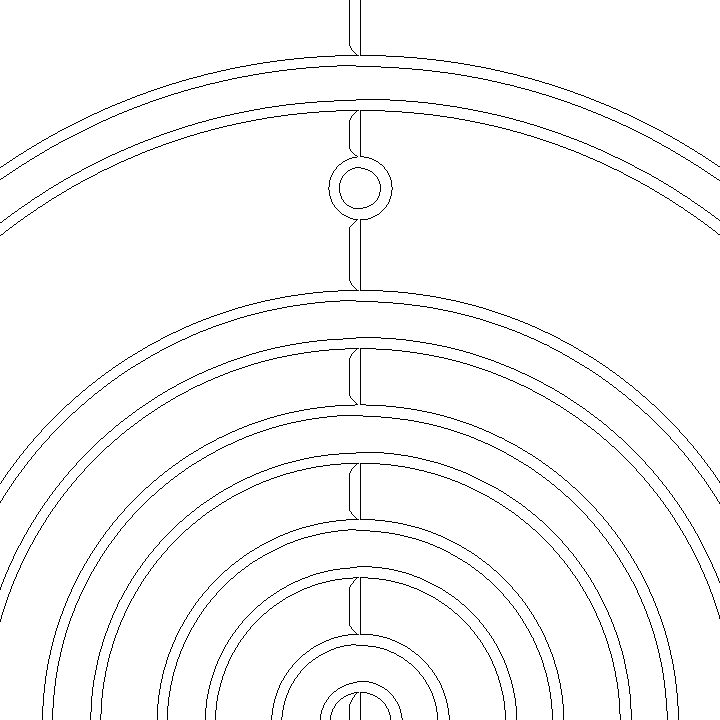
\includegraphics[width=\textwidth]
    {Gauss_cont_shadow}}
    \frame{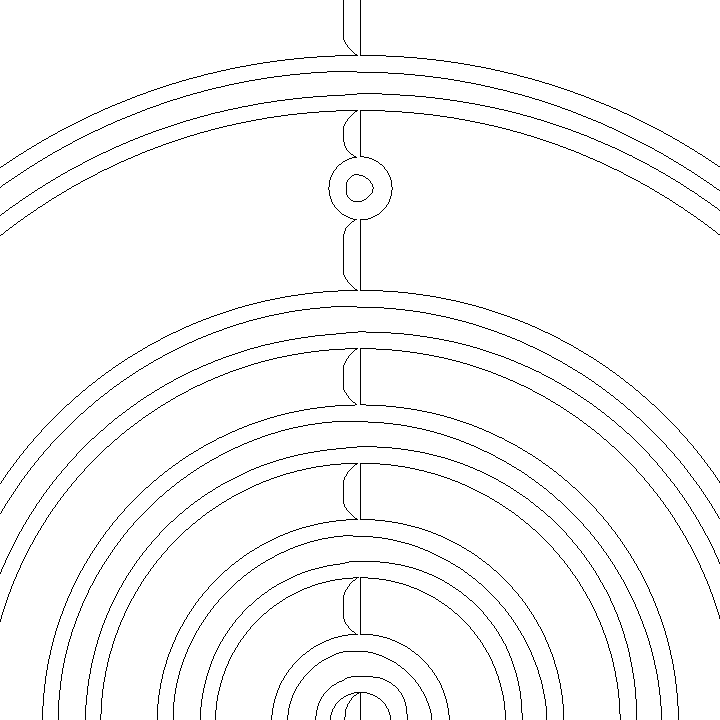
\includegraphics[width=\textwidth]
    {Mean_cont_shadow}}
    \caption{} 
\end{subfigure}\qquad
\begin{subfigure}[t]{0.15\textwidth}
    \frame{
\includegraphics[width=\textwidth]
    {tar_zoom_resolution}}
    \frame{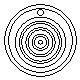
\includegraphics[width=\textwidth]
    {Otsu_cont_resolution}}
    \frame{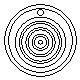
\includegraphics[width=\textwidth]
    {Riddler_cont_resolution}}
    \frame{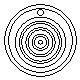
\includegraphics[width=\textwidth]
    {Yen_cont_resolution}}
    \frame{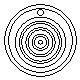
\includegraphics[width=\textwidth]
    {Li_cont_resolution}}
    \frame{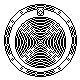
\includegraphics[width=\textwidth]
    {Niblack_cont_resolution}}
    \frame{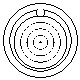
\includegraphics[width=\textwidth]
    {Sauvola_cont_resolution}}
    \frame{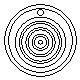
\includegraphics[width=\textwidth]
    {Bradley_cont_resolution}}
    \frame{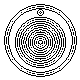
\includegraphics[width=\textwidth]
    {Gauss_cont_resolution}}
    \frame{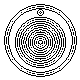
\includegraphics[width=\textwidth]
    {Mean_cont_resolution}}
    \caption{} 
\end{subfigure}\qquad
\begin{subfigure}[t]{0.15\textwidth}
    \frame{
\includegraphics[width=\textwidth]
    {tar_zoom_deformation}}
    \frame{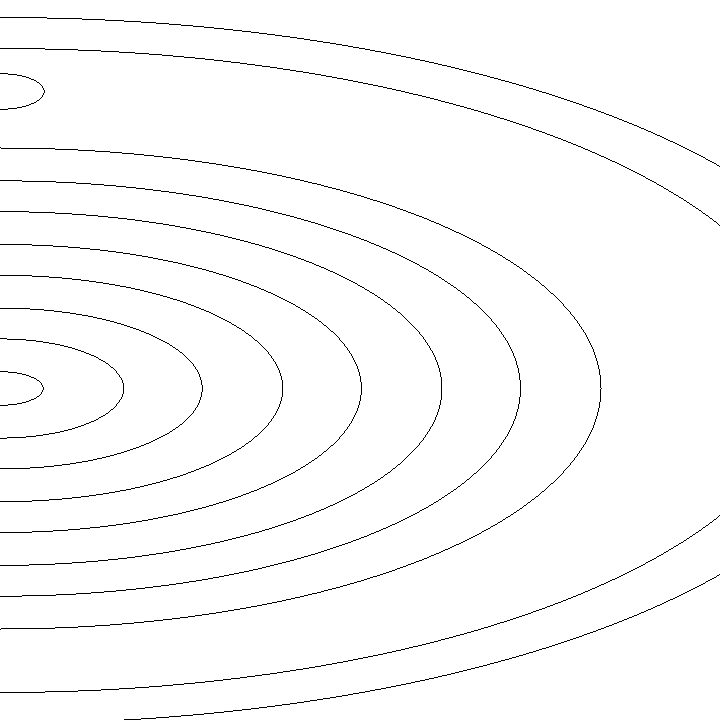
\includegraphics[width=\textwidth]
    {Otsu_cont_deformation}}
    \frame{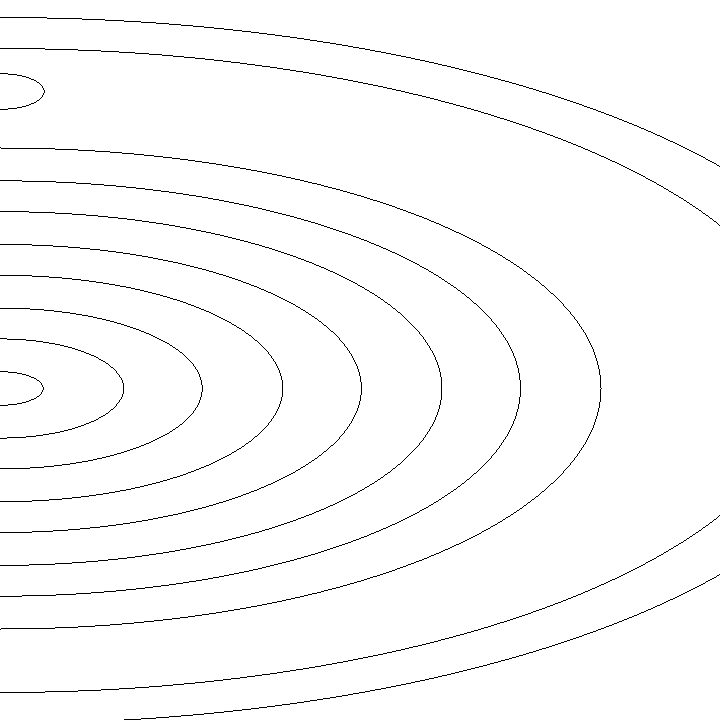
\includegraphics[width=\textwidth]
    {Riddler_cont_deformation}}
    \frame{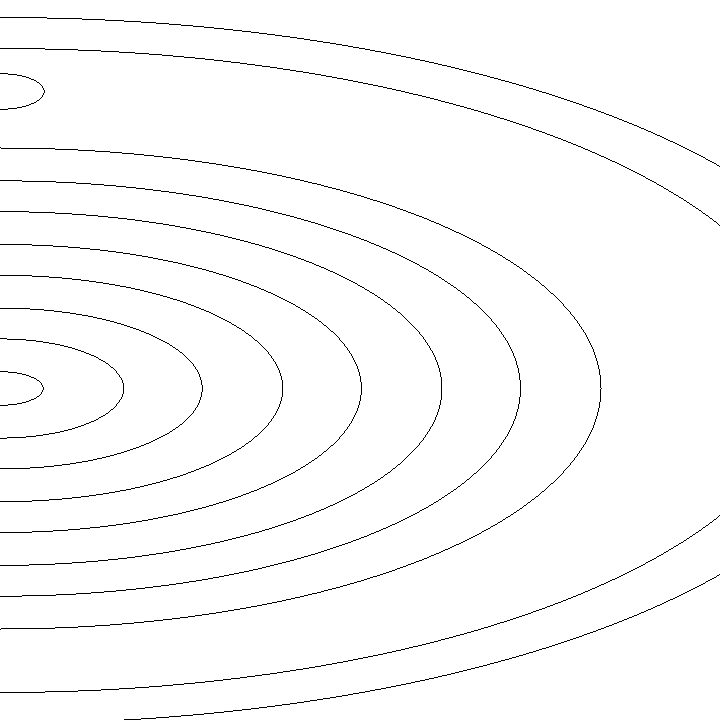
\includegraphics[width=\textwidth]
    {Yen_cont_deformation}}
    \frame{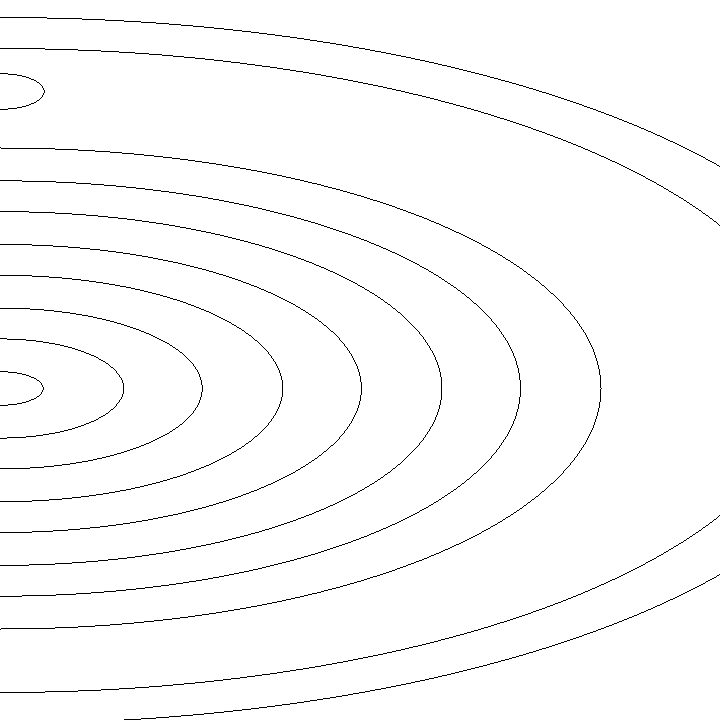
\includegraphics[width=\textwidth]
    {Li_cont_deformation}}
    \frame{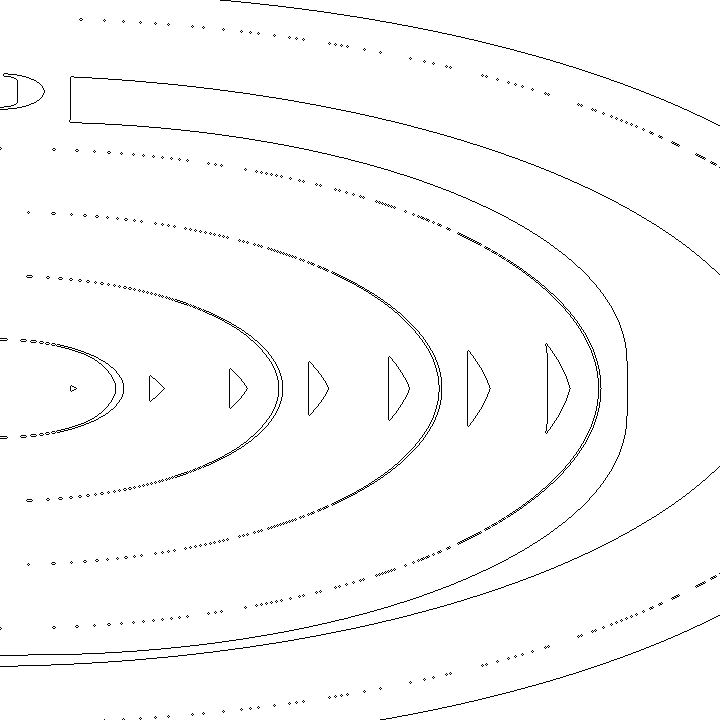
\includegraphics[width=\textwidth]
    {Niblack_cont_deformation}}
    \frame{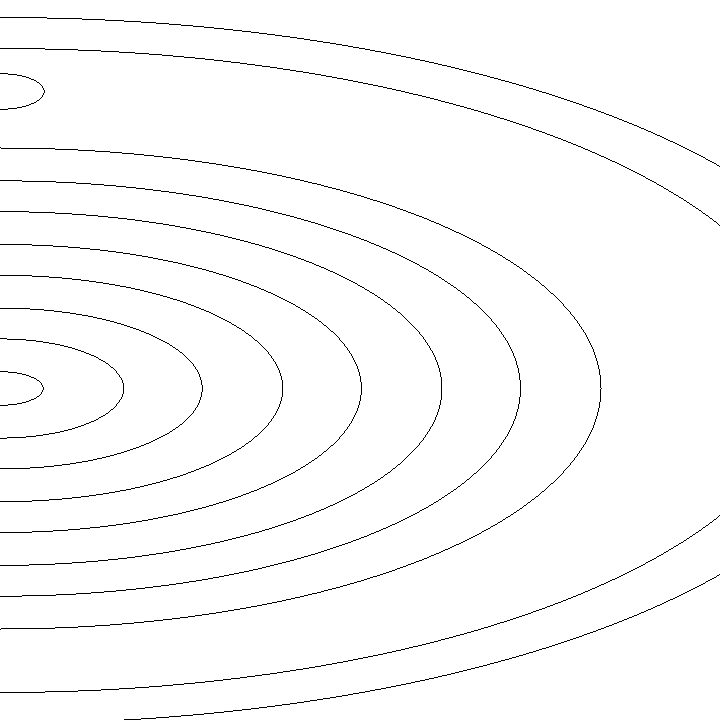
\includegraphics[width=\textwidth]
    {Sauvola_cont_deformation}}
    \frame{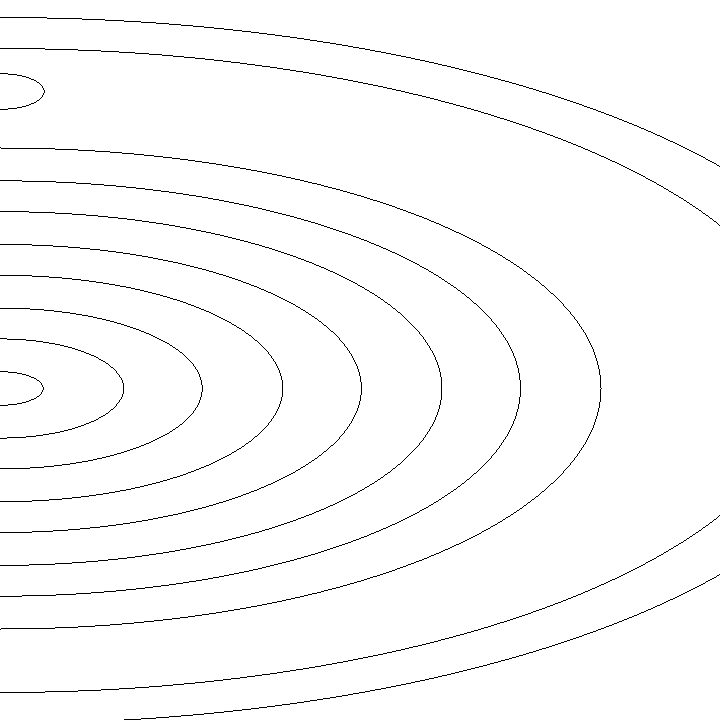
\includegraphics[width=\textwidth]
    {Bradley_cont_deformation}}
    \frame{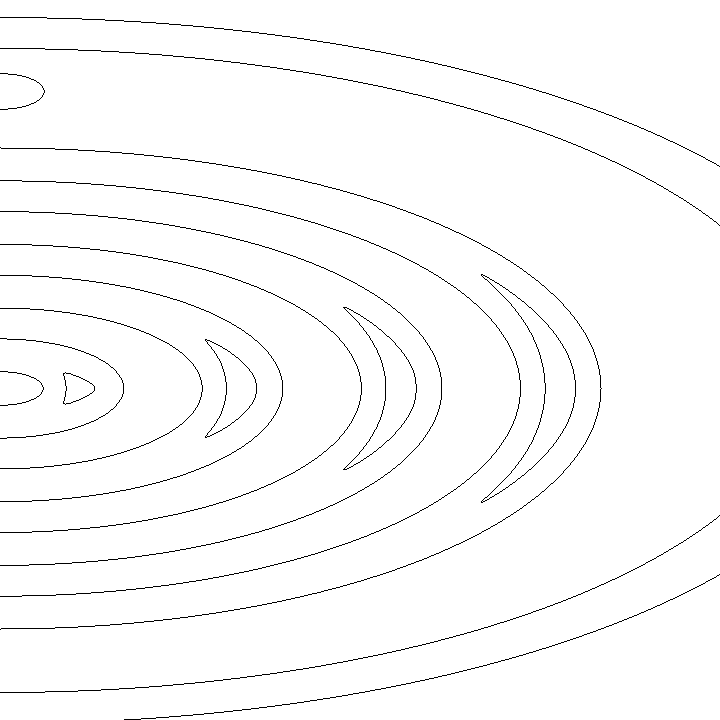
\includegraphics[width=\textwidth]
    {Gauss_cont_deformation}}
    \frame{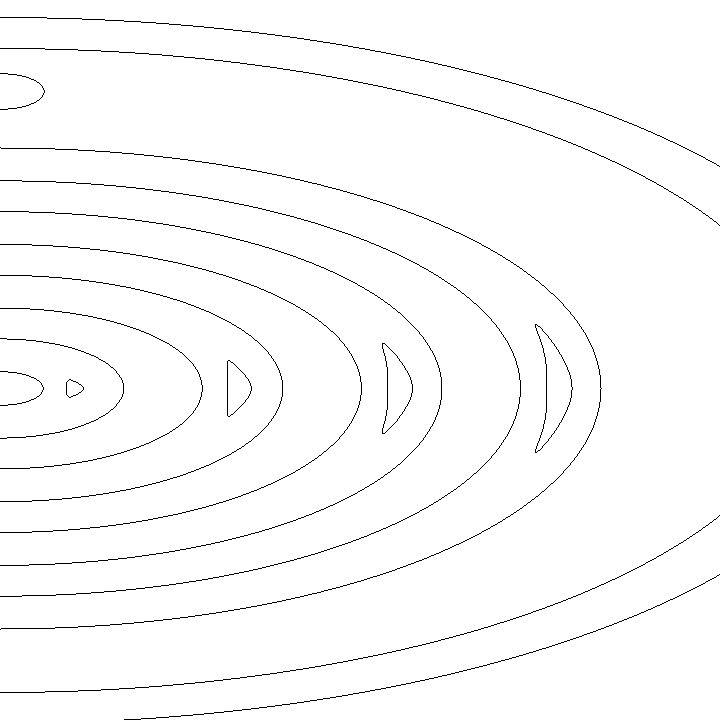
\includegraphics[width=\textwidth]
    {Mean_cont_deformation}}
    \caption{}  
\end{subfigure}
\caption{Thresholding methods result illustrations on synthetic images: \textbf{(a)} Noise, \textbf{(b)} Shadow, \textbf{(c)} Size and \textbf{(d)} Deformation degradations}\label{fig:thr_synth_comparison}
\end{figure}

We use nine the most representative thresholding to obtain a binary image, localize the image contours and evaluate which is the best facing image degradations showed in Fig. \ref{fig:tar_degradations}. Following the taxonomy proposed in \cite{Sezgin.Sankur:EI:2010}, we use the Otsu \cite{Otsu:SMC:1979} and the Riddler \cite{Ridler.Calvard:TSMC:1978} to evaluate the clustering-based methods, Yen\cite{Yen.Chang.ea:TIP:1995} and Li\cite{Li.Lee:ICPR:1993} as entropy-based methods, Niblack \cite{Niblack:ImageProcc:1986} and Sauvla \cite{Sauvola.Pietikainen:ICPR:2000} as local methods, the adaptive method proposed by Bradley \cite{Bradley.Roth:ACM:2007} and finally, the mean and Gaussian pixel distribution as spacial methods. 




The contours obtained applying each thresholding method are depicted in Fig. \ref{fig:thr_synth_comparison}. In this figure is appreciable that, depending on the situation the result is better or worse. However, at first glance, there is not one that works correctly in a general way.

\subsection{Thersholding Methods Evaluation}\label{sec:thresholding_evaluation}
The methodology proposed in \cite{BaquedanoA.:ESIEE:2017} works with the contour hierarchy heuristically to detect a landing target. As the landing target design has an unchanged number of concentric rings, the methodology consists in discriminating the contours that are not nested through conditional evaluations at each hierarchy level. The conditions are hierarchically dependent which means that the landing target detection is frustrated if the conditions are not strictly enforced.

We run this hierarchical algorithm on a database of synthetic images. The database contains the sixteen different landing targets perturbed by the image degradations of figure \ref{fig:tar_degradations}. 
The noise degradation is simulated by adding Gaussian noise with a mean of zero and a variable standard deviation from 0.02 to 0.2 where 0.02 is the minimum noise addition. 
The shadow perturbation is simulated shading the left-half of the image; the variation of the shadow is done between 0 and 1 where 0 indicates a darker left-half image. The last two degradations are related with the perspective and distance of the viewer (the camera). The change of scale is done scaling the landing target circles on a $640\times480$p image in an interval from 0 to 1, where 1 indicates real scale. Lastly, the perspective degradation is achieved by augmenting the proportion of one axis in an interval between 1 and 2, where to indicates the maximum deformation. We apply the maximum value degradation for the test.
 
We use the F1-score as metric to evaluate the accuracy of each thresholding method under different degradations. This metric has values between 0 and 1, where 1 is the best score and 0 the worst. Figure \ref{fig:degradations_graphs} shows the F1-score of the thresholding methods under the image degradations. The graphs show the behavior of the algorithm without an error-correction (gray bars) and with the use of the error-correction (black bars) described in appendix \ref{ch:target_description}.
\begin{figure}[h!]
    \centering
    \begin{subfigure}[b]{0.4\textwidth}
        \frame{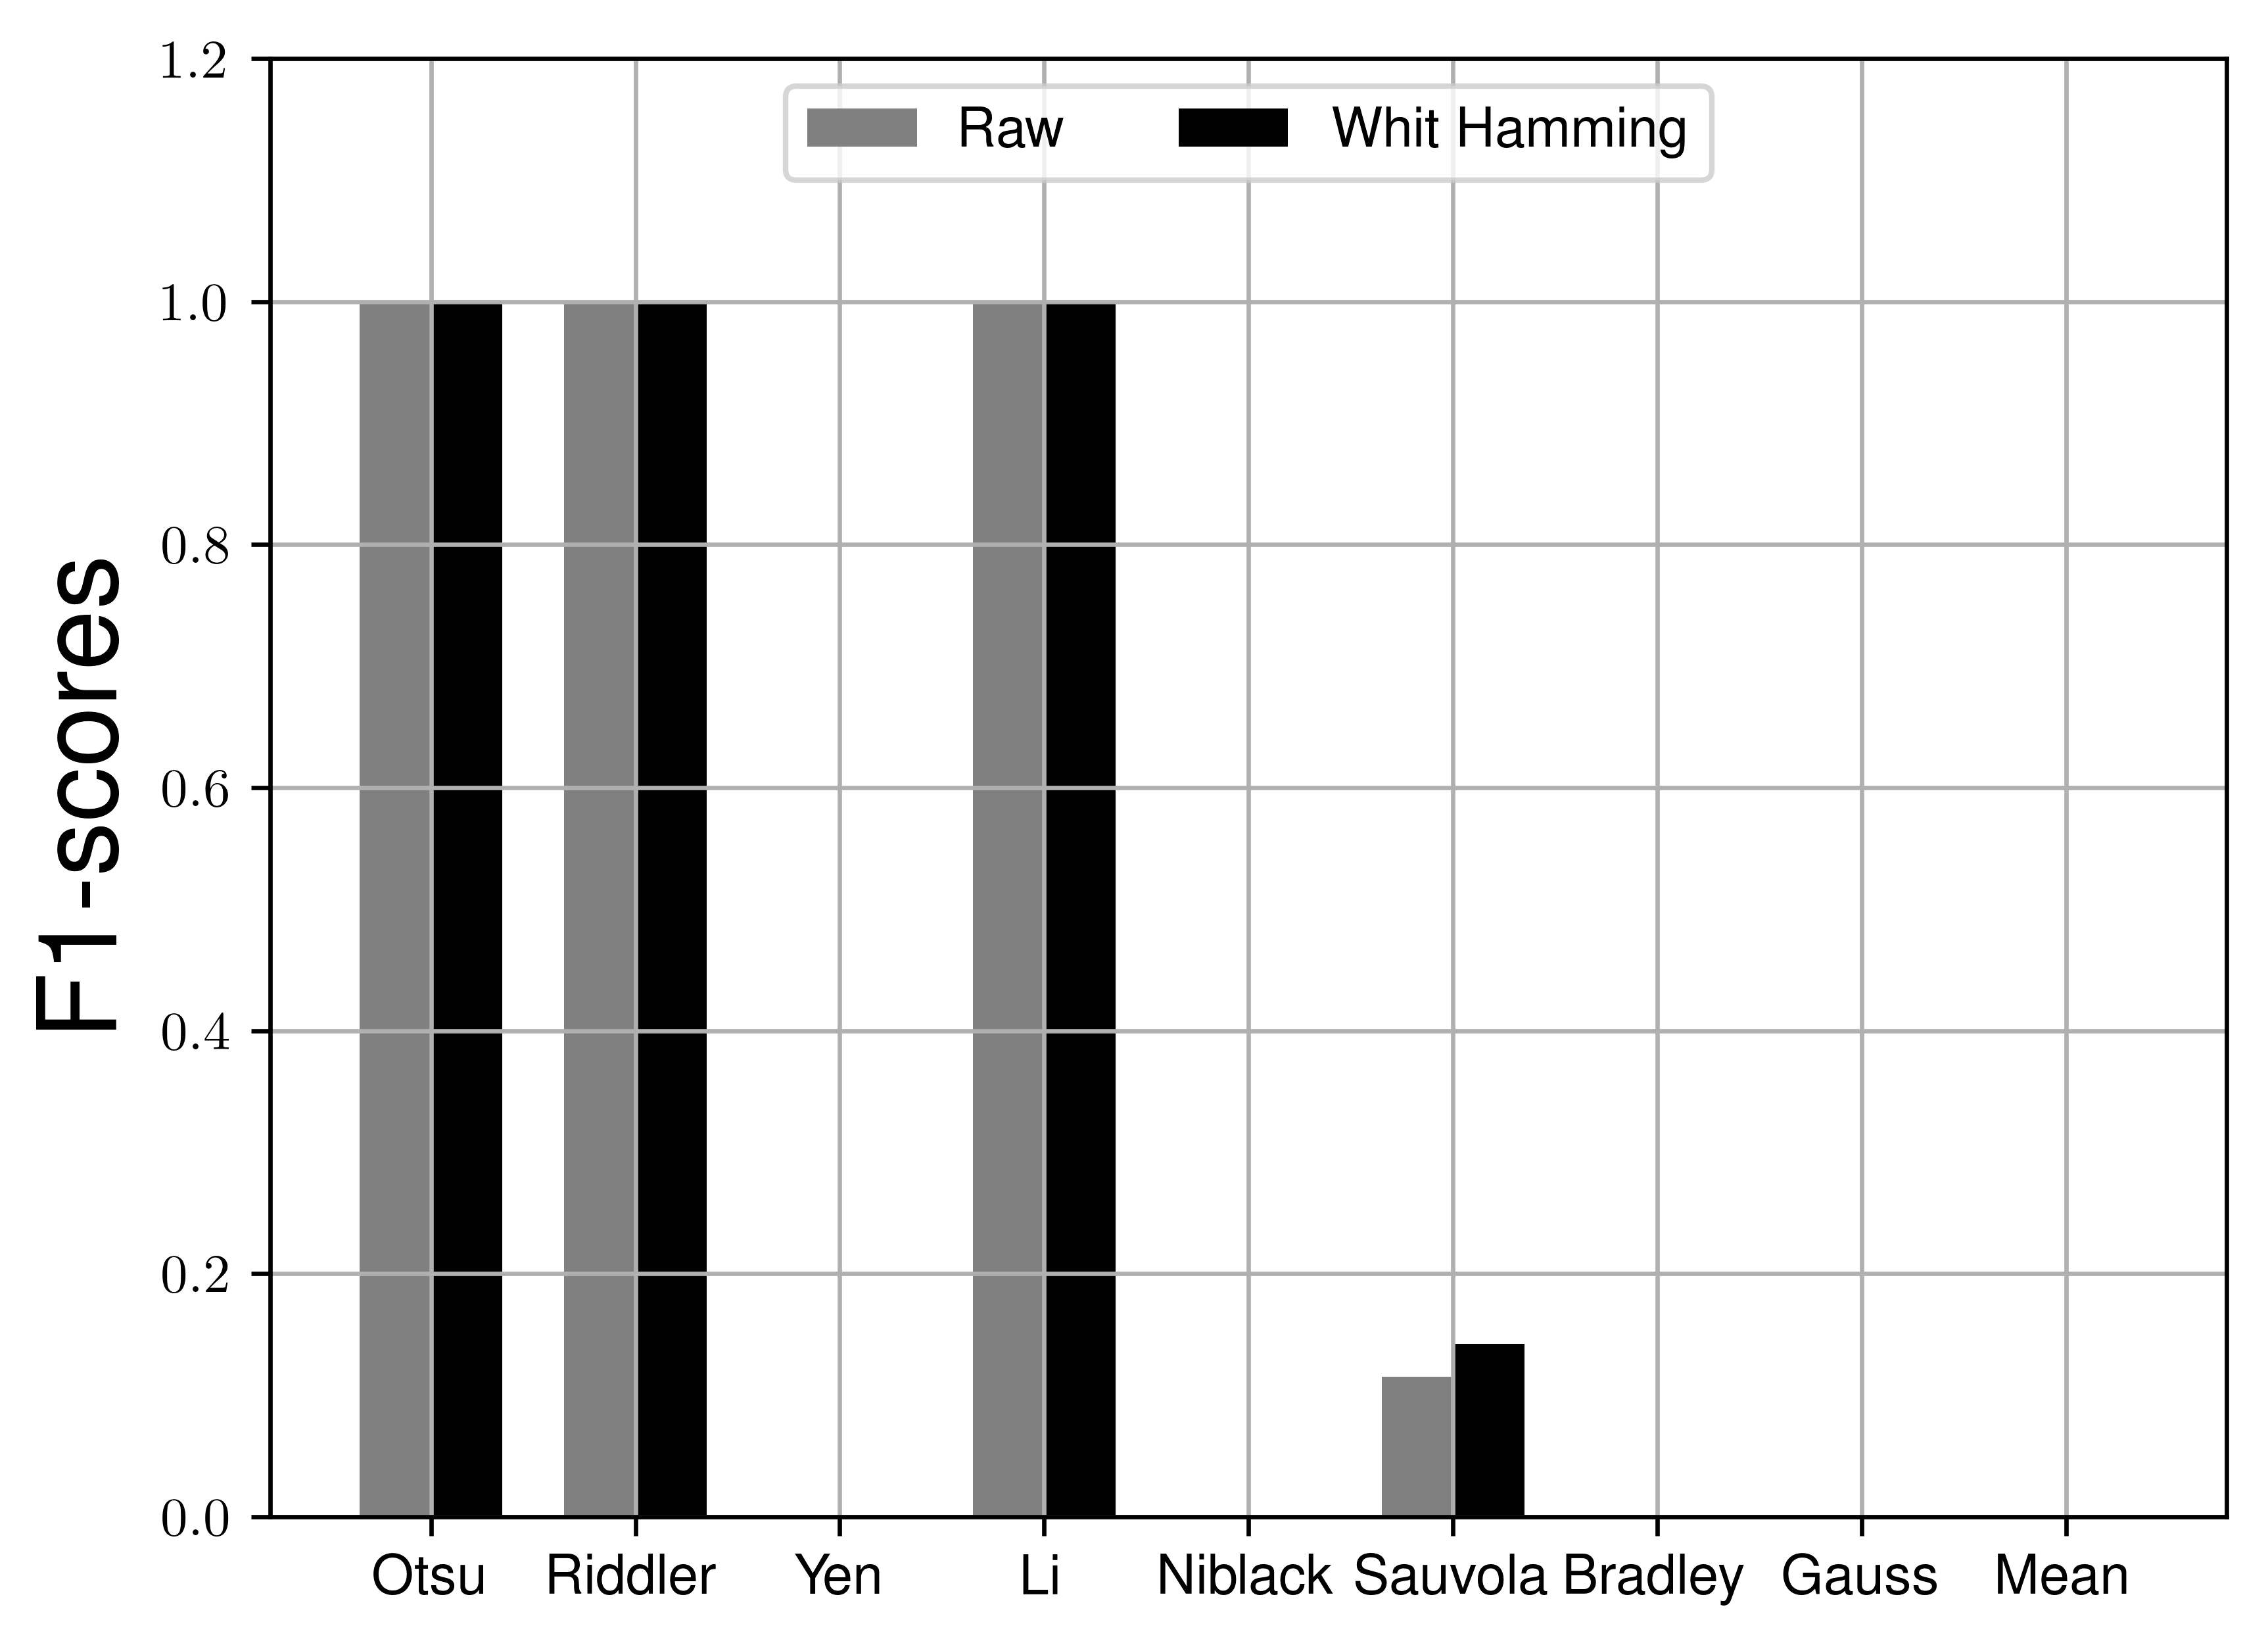
\includegraphics[width=\textwidth]{noise_comparison}}
        \caption{}
        \label{fig:noise_graph}
    \end{subfigure}
        ~ %add desired spacing between images, e. g. ~, \quad, \qquad, \hfill etc. 
      %(or a blank line to force the subfigure onto a new line)
    \begin{subfigure}[b]{0.4\textwidth}
        \frame{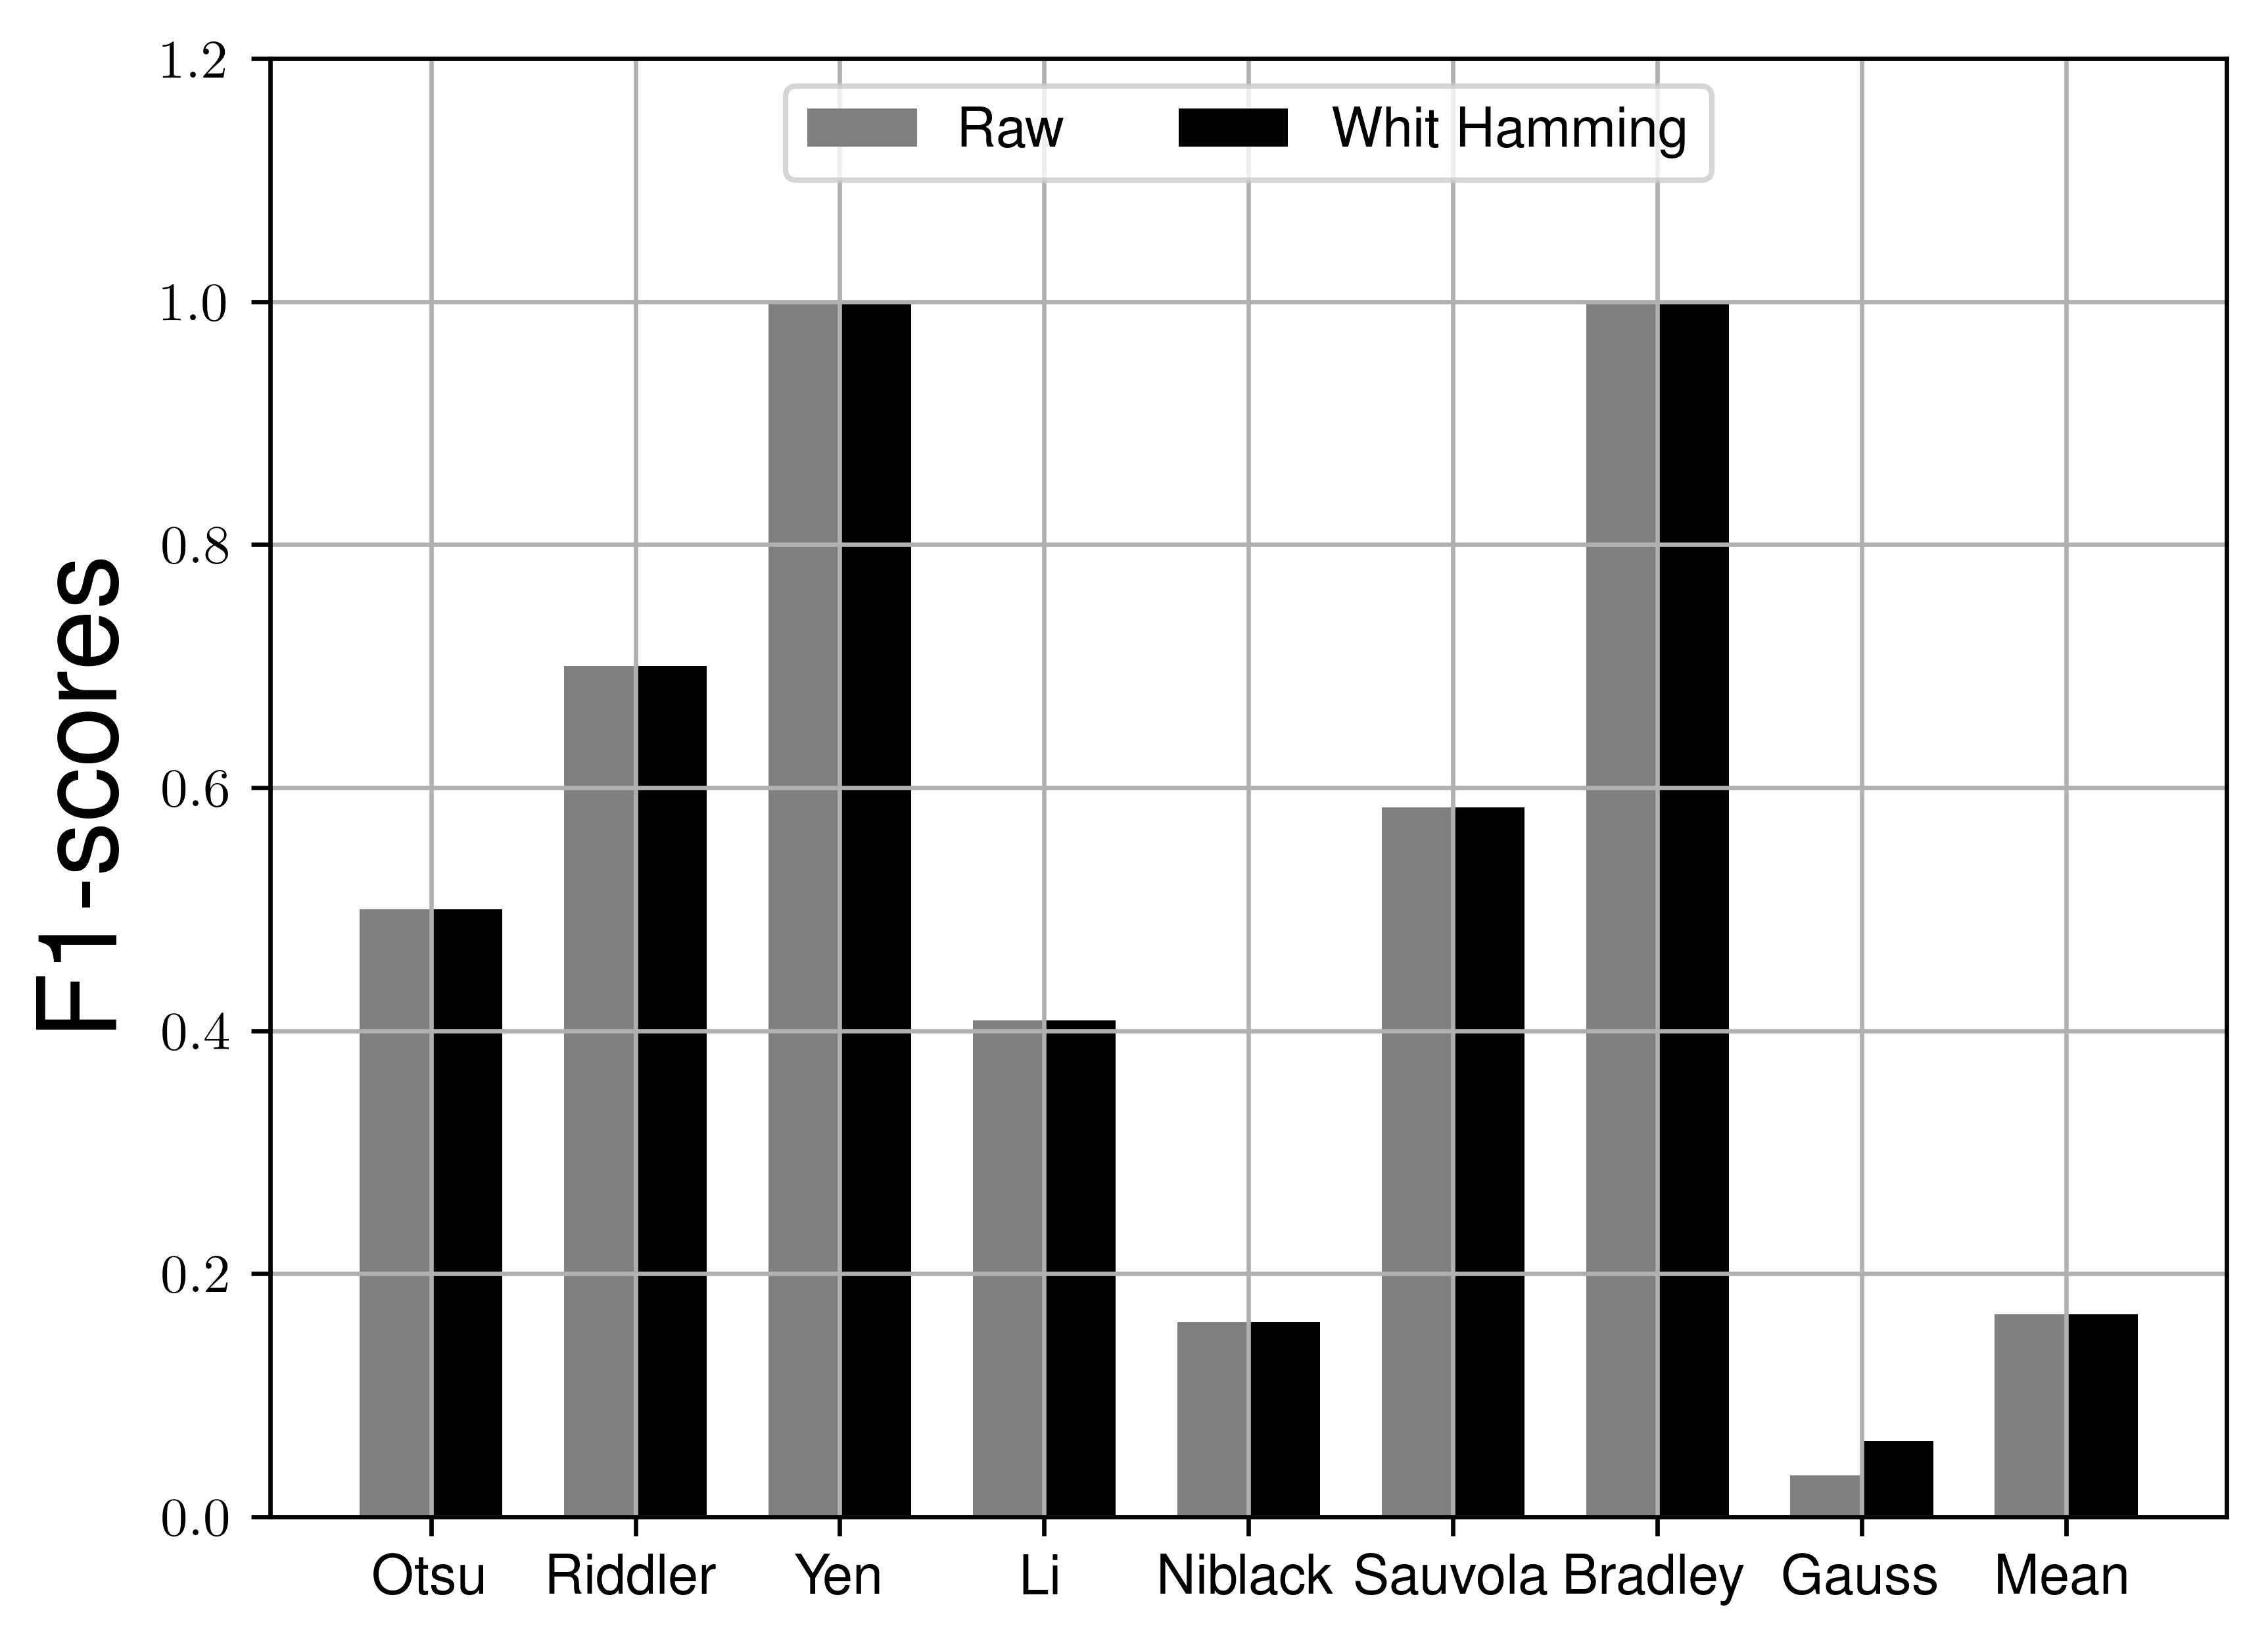
\includegraphics[width=\textwidth]{shade_comparison}}
        \caption{}
        \label{fig:shadow_graph}
    \end{subfigure}\\
        ~ %add desired spacing between images, e. g. ~, \quad, \qquad, \hfill etc. 
      %(or a blank line to force the subfigure onto a new line)
    \begin{subfigure}[b]{0.4\textwidth}
        \frame{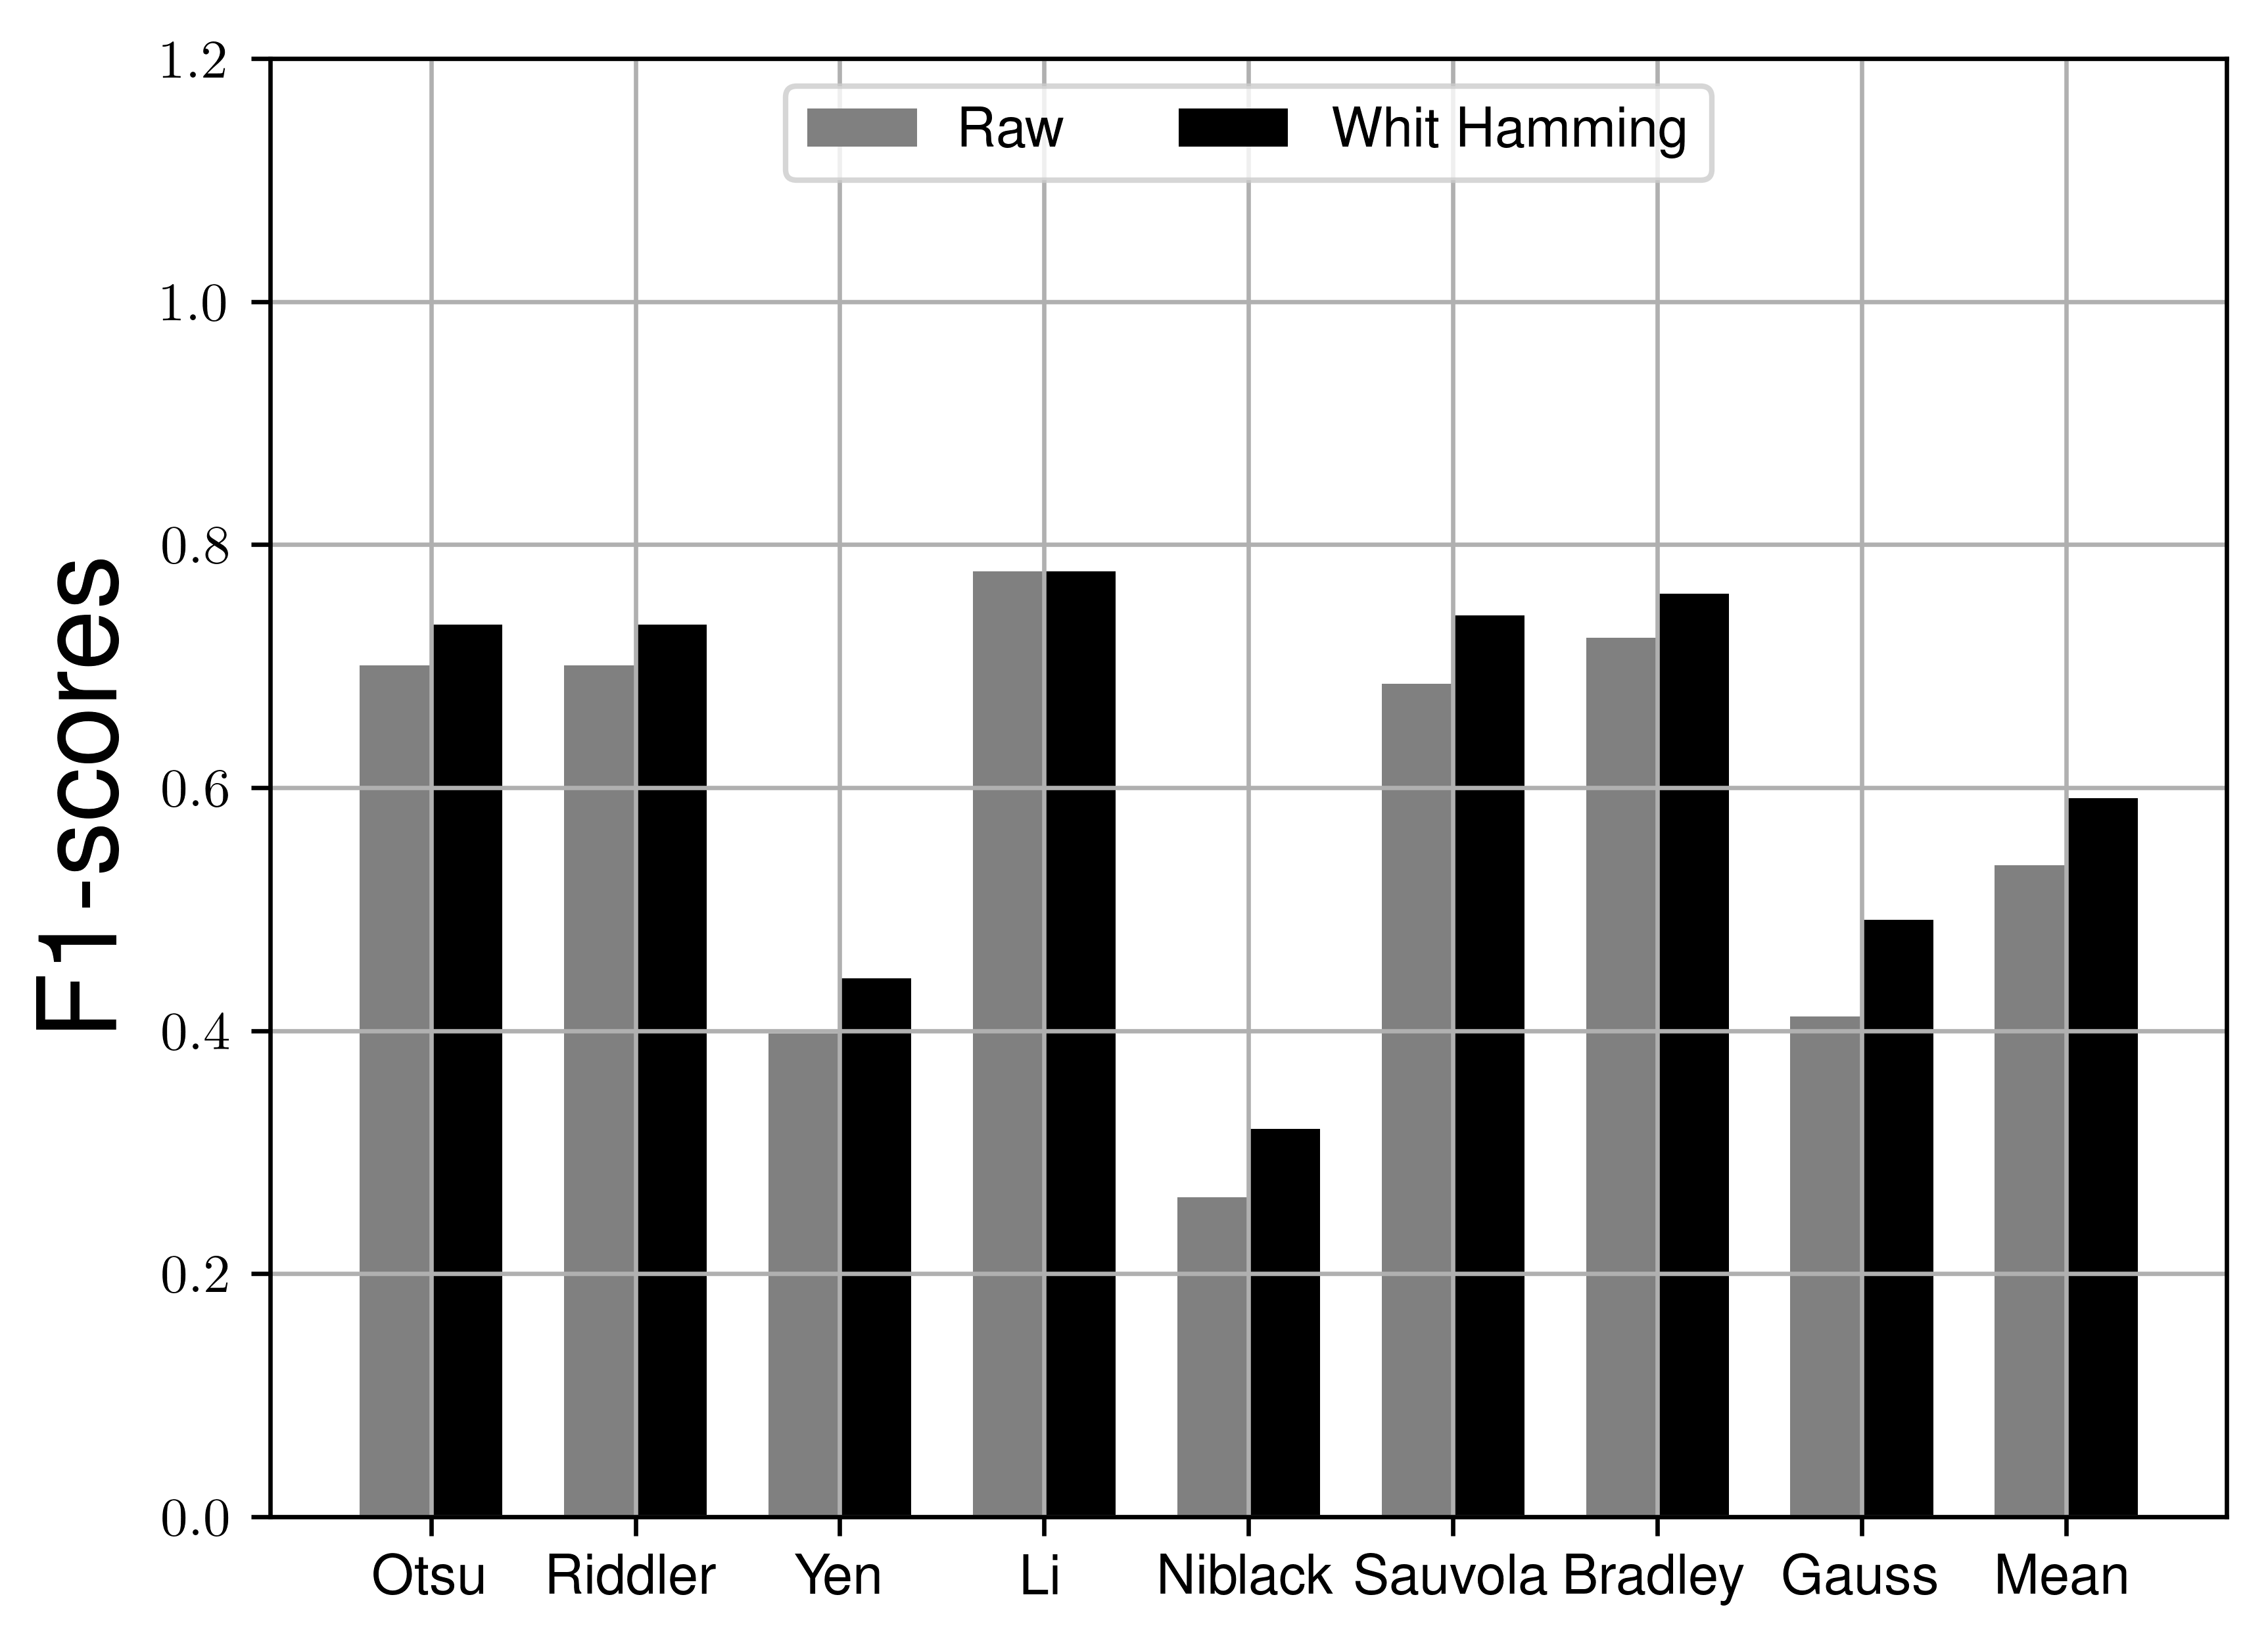
\includegraphics[width=\textwidth]{resolution_comparison}}
        \caption{}
        \label{fig:esolution_graph}
    \end{subfigure}
        ~ %add desired spacing between images, e. g. ~, \quad, \qquad, \hfill etc. 
      %(or a blank line to force the subfigure onto a new line)
    \begin{subfigure}[b]{0.4\textwidth}
        \frame{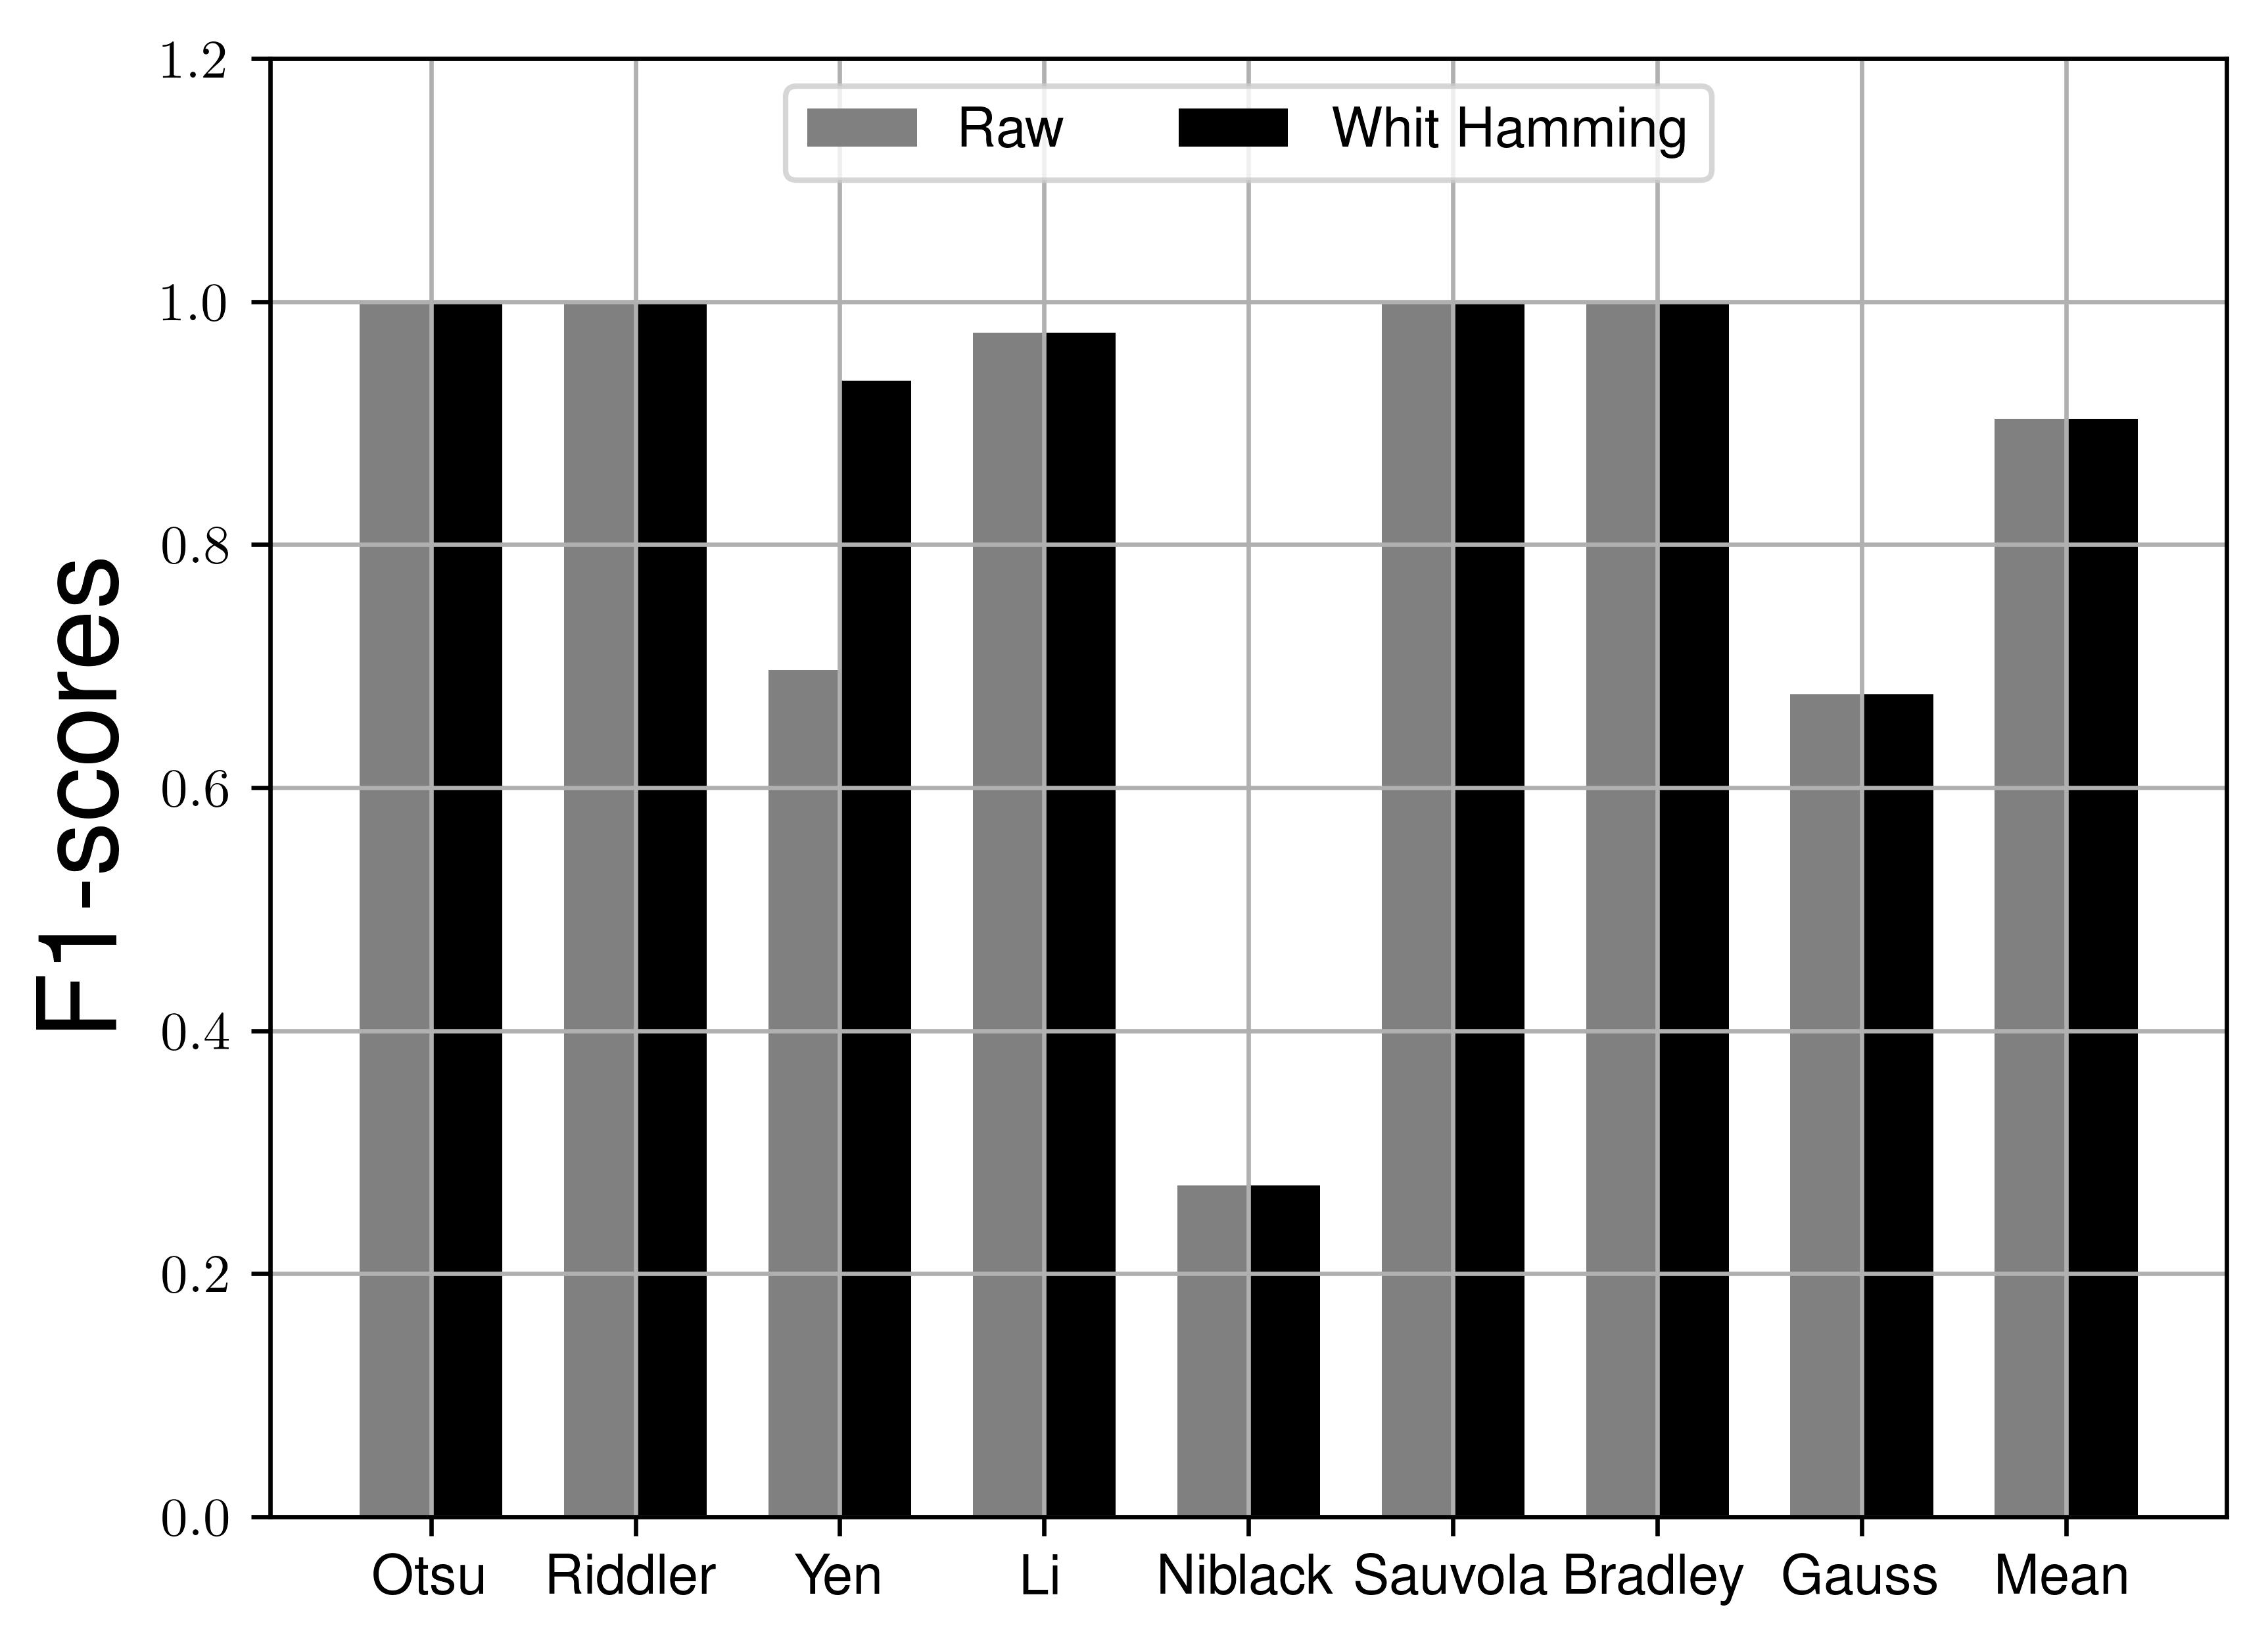
\includegraphics[width=\textwidth]{ellipse_comparison}}
        \caption{}
        \label{fig:deformation_graph}
    \end{subfigure}
    \caption{F1-score bar graphs: \textbf{(a)} Noise, \textbf{(b)} Shadow, \textbf{(c)} Change of size and \textbf{(d)} Perspectice deformation}\label{fig:degradations_graphs}
\end{figure}

The figure \ref{fig:thresholding_comp} and the F1-score graphs (Fig. \ref{fig:degradations_graphs}) shows that given the conditions where a landing target can be found, no thresholding method was robust to the set of perturbations. It is necessary to adjust parameters according to the condition to have acceptable results. Besides, we aim to recognize the landing targets in natural images where none, one or more landing targets can be present and the degradations are not isolated. The fig. \ref{fig:input_image} shows a landing target in an outdoor environment where the four degradations depicted in figure \ref{fig:tar_degradations} are present. We also show his histogram to highlight the saturation levels of the scene and the contours obtained with a representative method of each class of the taxonomy in \cite{Sezgin.Sankur:EI:2010}: clustering-based (fig. \ref{fig:otsu_th}), entropy-based (fig. \ref{fig:li_th}), spacial (fig. \ref{fig:gauss_th}) and local (fig. \ref{fig:sauvola_th}) thresholding methods.

\begin{figure}[h!]
    \centering
    \begin{subfigure}[b]{0.3\textwidth}
        \frame{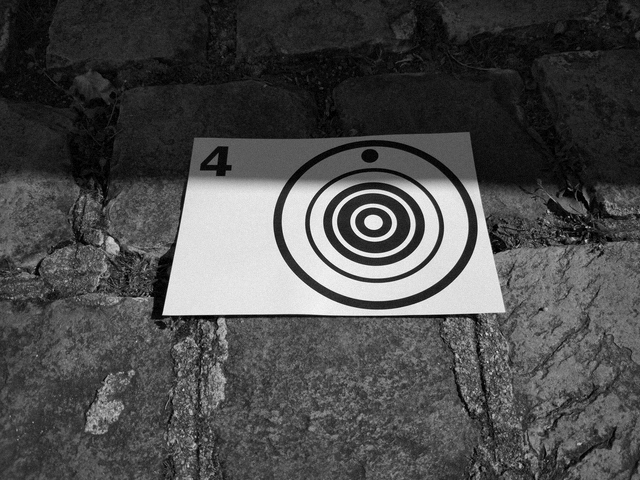
\includegraphics[width=\textwidth]{in_img_tar4}}
        \caption{Input image}
        \label{fig:input_image}
    \end{subfigure}
    ~ %add desired spacing between images, e. g. ~, \quad, \qquad, \hfill etc. 
      %(or a blank line to force the subfigure onto a new line)
    \begin{subfigure}[b]{0.3\textwidth}
        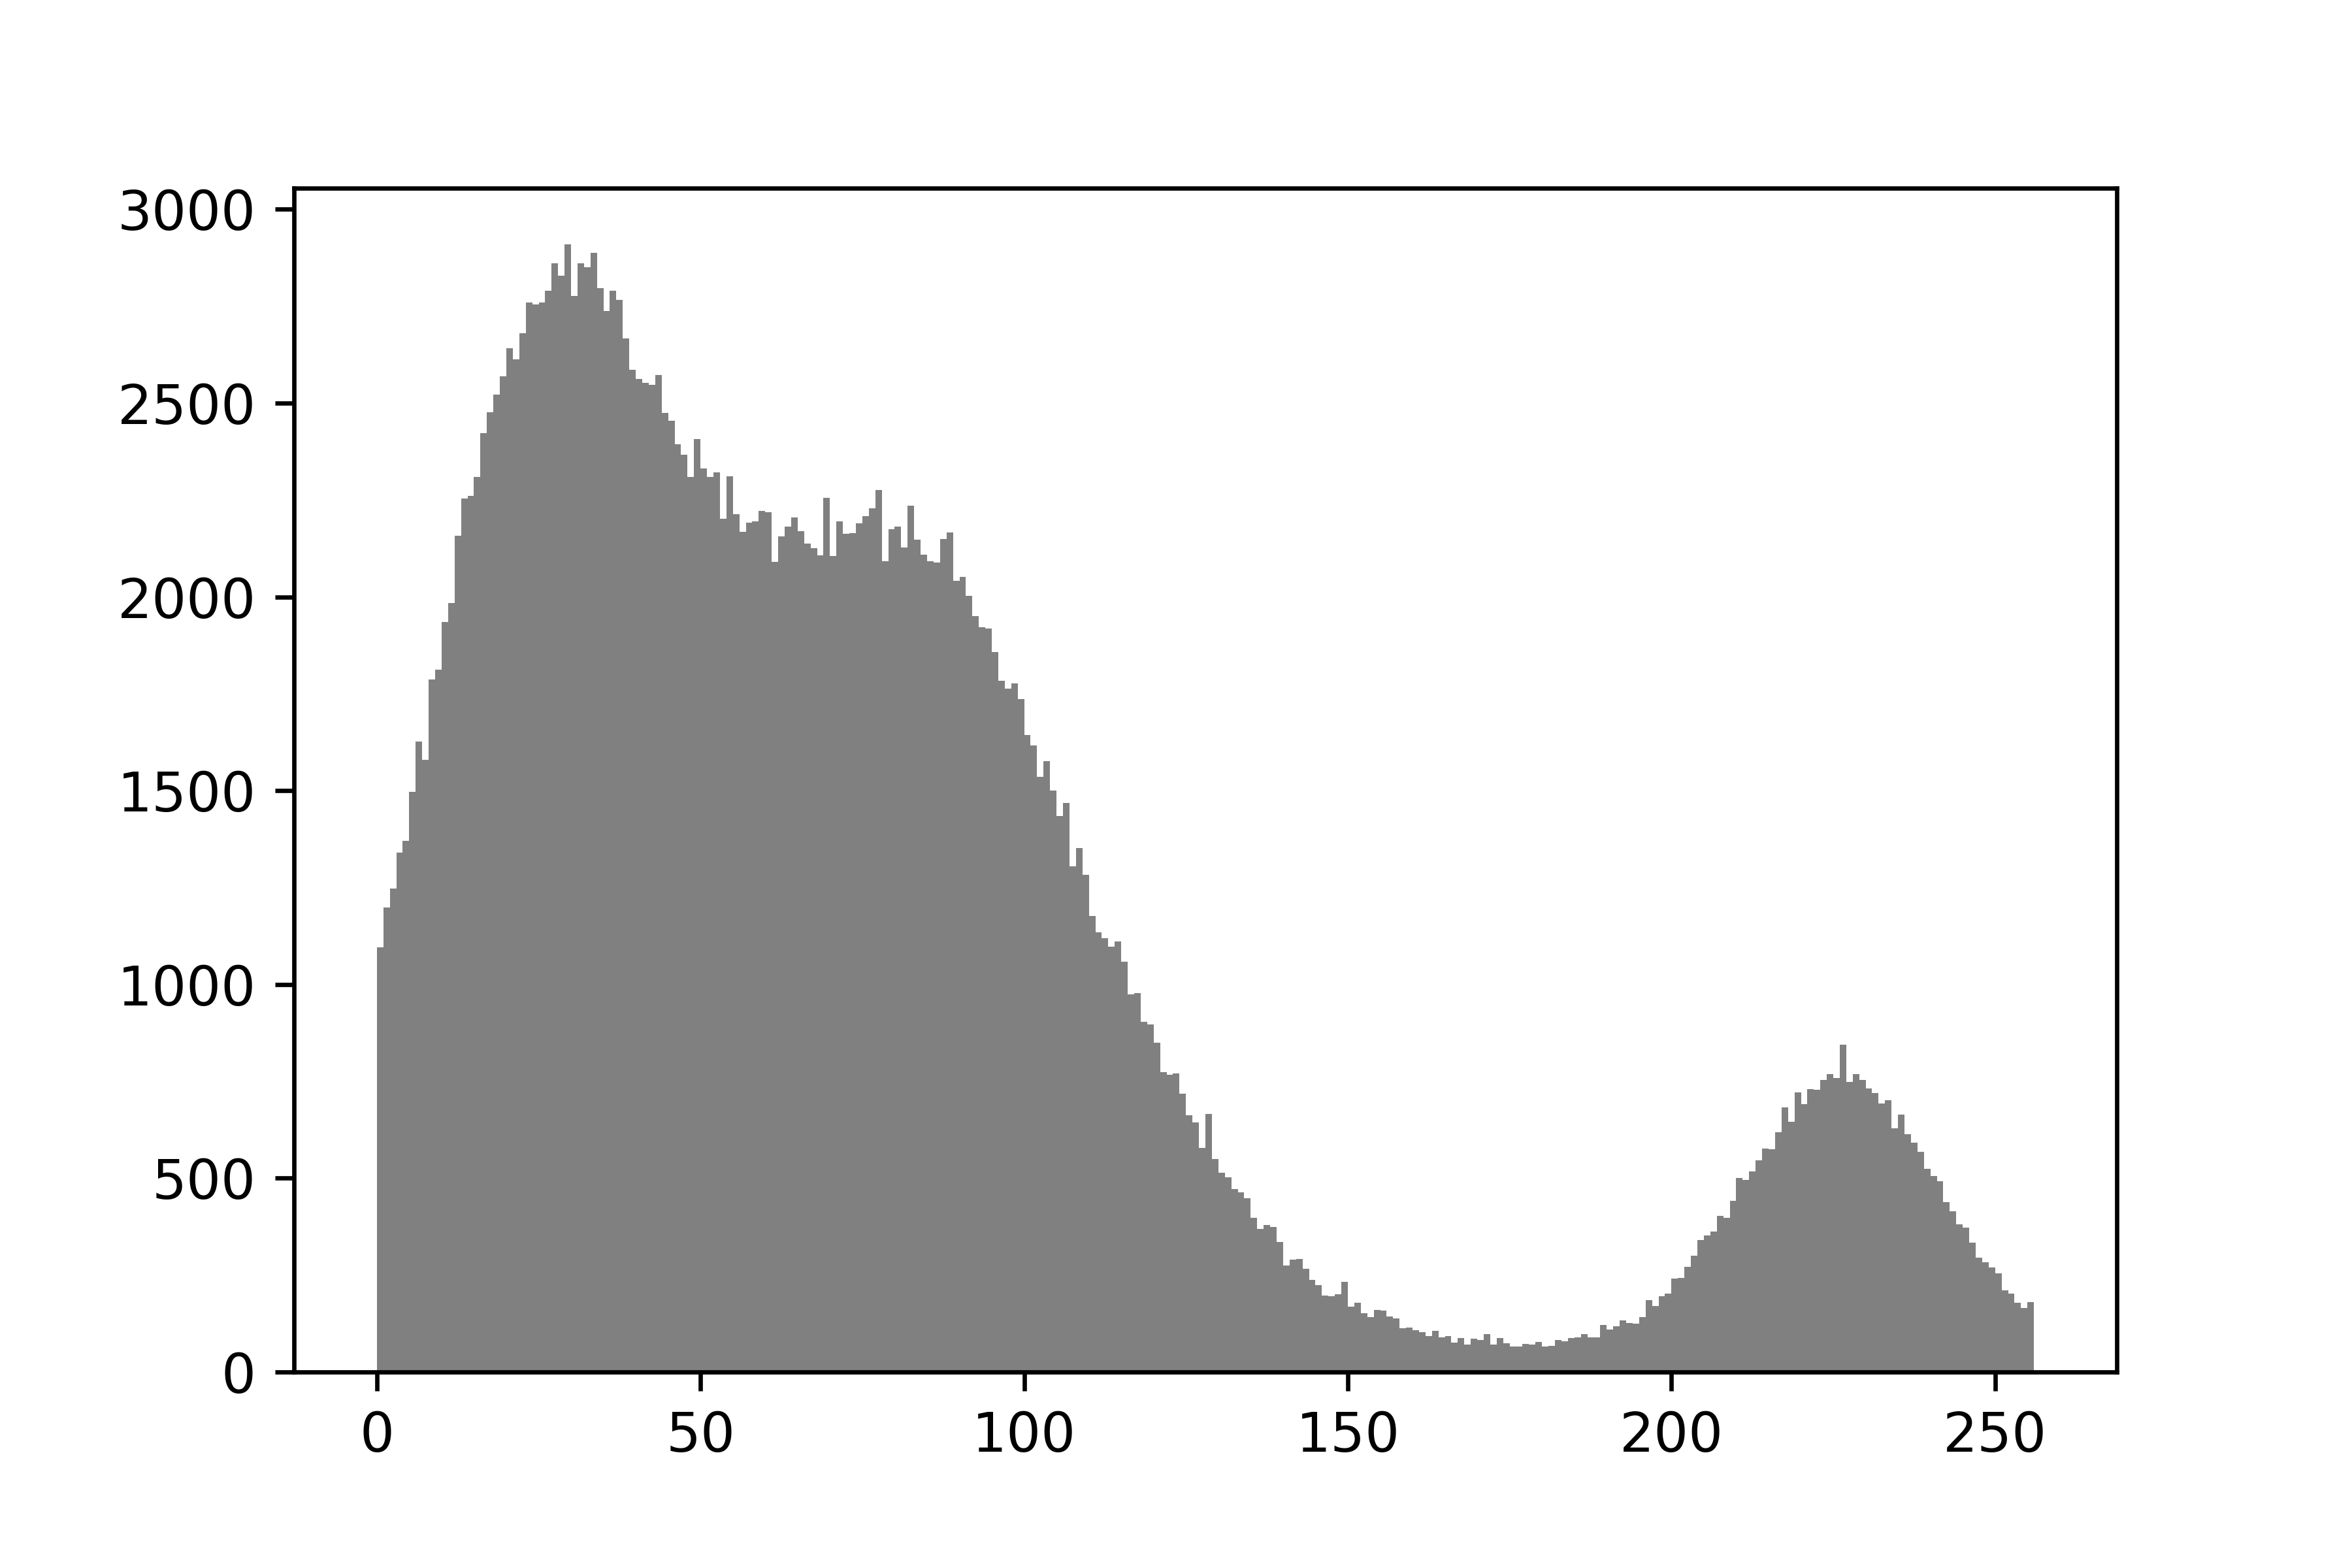
\includegraphics[width=\textwidth]{histogram}
        \caption{Histogram of input image}
        \label{fig:histogram}
    \end{subfigure}\\
        ~ %add desired spacing between images, e. g. ~, \quad, \qquad, \hfill etc. 
      %(or a blank line to force the subfigure onto a new line)
    \begin{subfigure}[b]{0.16\textwidth}
        \frame{\includegraphics[width=\textwidth]{in_img_tar4_zoom}}
        \caption{Zoom}
        \label{fig:tar4_zoom}
    \end{subfigure}
        ~ %add desired spacing between images, e. g. ~, \quad, \qquad, \hfill etc. 
      %(or a blank line to force the subfigure onto a new line)
    \begin{subfigure}[b]{0.16\textwidth}
        \frame{\includegraphics[width=\textwidth]{Otsu_cont}}
        \caption{Otsu}
        \label{fig:otsu_th}
    \end{subfigure}
        ~ %add desired spacing between images, e. g. ~, \quad, \qquad, \hfill etc. 
      %(or a blank line to force the subfigure onto a new line)
    \begin{subfigure}[b]{0.16\textwidth}
        \frame{\includegraphics[width=\textwidth]{Li_cont}}
        \caption{Li}
        \label{fig:li_th}
    \end{subfigure}
        ~ %add desired spacing between images, e. g. ~, \quad, \qquad, \hfill etc. 
      %(or a blank line to force the subfigure onto a new line)
    \begin{subfigure}[b]{0.16\textwidth}
        \frame{\includegraphics[width=\textwidth]{Gauss_cont}}
        \caption{Gauss }
        \label{fig:gauss_th}
    \end{subfigure}
        ~ %add desired spacing between images, e. g. ~, \quad, \qquad, \hfill etc. 
      %(or a blank line to force the subfigure onto a new line)
    \begin{subfigure}[b]{0.16\textwidth}
        \frame{\includegraphics[width=\textwidth]{Sauvola_cont}}
        \caption{Sauvola}
        \label{fig:sauvola_th}
    \end{subfigure}
    \caption{Landing target under non-controlled illumination conditions and the controus obtained with some thresholding methods}\label{fig:thresholding_comp}
\end{figure}

\section{Gestalt Theory in Image Analysis}

\subsection{Human perception principles and \textit{a contrario} methods}


\section{Unsupervised Perception Model}

\subsection{Non-accidentalness Estimation}\label{subsec:Helmholtz}

\subsubsection{Contour Detection}\label{subsubsec:muiltiscale}
Instead of using a thresholding method, we obtain the image without fixing any parameter. The use of the Marr-Hildreth \cite{Marr.Hildreth:PRS:1980} operator guarantees to find continuous and closed contours eliminating the possible noise in the image, while the contours of objects remain unchanged in the presence of shadows. This technique convolves the intensity image $f$ with the 2-D Laplacian of Gaussian operator $\nabla^{2} G(x, y,\sigma)$ and generates an image, 
\begin{eqnarray}\label{eq:LoG}
l_\sigma =  \nabla^{2} G(\sigma)\ast f
\end{eqnarray}
in which we localize the zero-crossings. 

The parameter $\sigma$ in eq. (\ref{eq:LoG}) permits to control the amount of image smoothing, but also acts as scale parameter, that when varies, it generates different scale-space images. Since no single filter can be optimal simultaneously at all scales \cite{Marr.Hildreth:PRS:1980}, we use a multi-scale analysis \cite{Witkin:ICASSP:1984} to detect the zero-crossings in $l_\sigma$ at different scale-spaces to minimize the risk that some contour of interest is not detected. The image $l_\sigma$ from eq. (\ref{eq:LoG}) contains a set of contours $\mathcal{L}_{\sigma}=\{L_{i}^{\sigma}, \enspace i=0, 1, \ldots, N\}$ for a given scale $\sigma$. Then, 
\begin{eqnarray}\label{eq:all_ctns_set}
\mathcal{L}=\bigcup\limits_{\sigma}  L_{\sigma}
\end{eqnarray}
represents all the contours of an image obtained at different scale-spaces. Figure \ref{fig:all_cnts} shows the set of contours $\mathcal{L}$ found for $\sigma=[1,2,3]$. Besides, it is also appreciated that at a fine scale (Fig. \ref{fig:cnts_scale1}) we can see more characteristics of the objects, i.e., there are more contours. Conversely, in coarse scales (Fig. \ref{fig:cnts_scale3}), due to the smoothing, there is a spatial distortion, and fewer contours appear. However, those contours that had already appeared at a coarse scale, will not disappear. Then, exist the probability that those contours that spatially coincide on two or more scales belong to a change of intensity generated by the border of an object. 
\begin{figure}[h]
    \centering
    \begin{subfigure}[b]{0.3\textwidth}
        \frame{\includegraphics[width=\textwidth]{cnts_sig1_tar4}}
        \caption{$\mathcal{L}_{\sigma}$ for $\sigma=1$}
        \label{fig:cnts_scale1}
    \end{subfigure}
    ~ %add desired spacing between images, e. g. ~, \quad, \qquad, \hfill etc. 
      %(or a blank line to force the subfigure onto a new line)
    \begin{subfigure}[b]{0.3\textwidth}
        \frame{\includegraphics[width=\textwidth]{cnts_sig3_tar4}}
        \caption{$\mathcal{L}_{\sigma}$ for $\sigma=2$}
        \label{fig:cnts_scale2}
    \end{subfigure}\\
        ~ %add desired spacing between images, e. g. ~, \quad, \qquad, \hfill etc. 
      %(or a blank line to force the subfigure onto a new line)
    \begin{subfigure}[b]{0.3\textwidth}
        \frame{\includegraphics[width=\textwidth]{cnts_sig3_tar4}}
        \caption{$\mathcal{L}_{\sigma}$ for $\sigma=3$}
        \label{fig:cnts_scale3}
    \end{subfigure}
        ~ %add desired spacing between images, e. g. ~, \quad, \qquad, \hfill etc. 
      %(or a blank line to force the subfigure onto a new line)
    \begin{subfigure}[b]{0.3\textwidth}
        \frame{\includegraphics[width=\textwidth]{all_cnts_tar4}}
        \caption{Set $\mathcal{L}$ for $\sigma=[1, 2 ,3]$}
        \label{fig:all_cnts}
    \end{subfigure}
    \caption{The image contours found at three different scales joined in the set $\mathcal{L}$}\label{fig:multiscale_cnts}
\end{figure}

\subsubsection{Multi-feature Space}\label{subsec:multispace}
The Helmholtz principle states that meaningful characteristics appear as large deviations from randomness and that is how the human perception automatically works to identify an object \cite{Attneave:PR:1954}. The a contrario model proposed in \cite{Desolneux.Moisan.ea:Gestalt:2008}, formulates this principle statistically by setting the number of false alarms (NFA) below some acceptable level; however, this method cannot be easily extended to more complex shapes. Instead of setting the NFA, we use the RX detector \cite{Reed.Yu:TASSP:1990} to detect outliers. Initially called the constant false alarms rate detection algorithm (CFAR) it can detect the presence of a know signal pattern in several signal-plus-noise channels. For that, it uses a $N\times Q$ multi-variable space $Z=[Z_{1}, \ldots, Z_{Q}]$ with $Q$  observation vectors of dimension $N$. In our approach, the primitive is a closed contour. We build the multi-variable space with observations based on internal (geometrical features, e.g., circularity, roundness, area, perimeter) and external (e.g., mean gradient intensity,  intensity inner area) properties of the contours.

Let $L_{i} \in \mathcal{L}$ be a contour, $A_{i}$ its area and $P_{i}$ its perimeter; we compute the circularity eq.(\ref{eq:circuarity}) and the mean gradient intensity eq. (\ref{eq:mean_gradient}) to build the multi-variable space $Z=[Z_{1}, Z_{2}]$. 

\begin{eqnarray}
Z_{1}&=&\left[\frac{4\pi A_{i}}{P_{i}^2}, \enspace i=0, \ldots, N\right]^T,  \enspace N = card(\mathcal{L}) \label{eq:circuarity}  \\ 
Z_{2}&=&\left[\frac{1}{P_{i}}\sum\limits_{x \in L_{i}} \mid\nabla f(x) \mid, \enspace L_{i} \in \mathcal{L}\right]^T  \label{eq:mean_gradient}
\end{eqnarray}

\subsubsection{RX Detector}\label{subsec:rx_detector}
The RX anomaly detector \cite{Reed.Yu:TASSP:1990} is commonly used to detect outliers on such data. The space $Z$ models the set of contours $\mathcal{L}$ with $Q=2$ feature vectors describing the circularity eq. (\ref{eq:circuarity}) and the mean gradient intensity eq.(\ref{eq:mean_gradient}). The RX detector gives an anomaly score to each contour taking into account the mean of the distribution and covariance between the $Q$-features through the Mahalanobis distance,
\begin{eqnarray}\label{eq:RX_detector}
y_{i}= (z_{i}-\mu_{Z})^{T}\Sigma^{-1}_{Z}(z_{i}-\mu_{Z})
\end{eqnarray}
where $\mu_{Z}=[\mathrm{E}[z_{1}], \ldots, \mathrm{E}[z_{N}]]^T$ is the  observations mean vector and $\Sigma^{-1}_{Z}$ the $N\times Q$ covariance matrix of the data. If the data have normal random distribution, then the score vector $Y=[y_{i}, \ldots, y_{N}]$ follows a chi-square distribution $\chi^{2}_{Q}(\varphi)$ with $Q$ degrees of freedom, where $\varphi$ is a confidence level \cite{Lu.Chen.ea:IJAIT:2004}. The value of $\chi^{2}_{Q}(\varphi)$ with a confidence value $\varphi=99.9\%$ operates as a threshold to identify all contours that behave as outliers in the multi-variable distribution. In our case, the contours belonging to a landing target appear as outliers in the vast majority of random contours belonging to the background.

With the previous strategy we preserve the anomalous contours having a value of mean gradient and circularity deviating from the principal mode of the distribution in the set $\widetilde{\mathcal{L}}=\{L_{i}\mid y_{i}>\chi^{2}_{Q}(\varphi)\}$. $\chi^{2}_{Q}(\varphi)$ is the value of the cumulative distribution at the confidence level $\varphi$ and $\widetilde{\mathcal{L}} \subset \mathcal{L}$. It is essential to mention the importance of multi-scale contour detection of section \ref{subsec:multispace}; because it increases the number of samples in Z, allowing to build a richer multi-variable space.

In the set $\widetilde{\mathcal{L}}$ some contours make not part of a landing target. For example, in the figure \ref{fig:rx_cnts}, we can see that the paper sheet contours remain because they have a high value of circularity. The same occurs with the contours of those objects with an important value of mean gradient, as the number 4 at the top-left of the sheet or the rock textures of the background.
\begin{figure}[h]
    \centering
    \frame{\includegraphics[width=0.35\linewidth]{rx_cnts_tar4}}
    \caption{The contours from Fig. \ref{fig:all_cnts} that behave as outliers in the multi-feature space $Z$ with a confidence value of $\varphi=99.9\%$}
    \label{fig:rx_cnts}
\end{figure}

\subsection{Gestalt Laws of Grouping}\label{subsec:Gestalt}
We use the Gestalt theory \cite{Wertheimer:Psycologische:1923} to group the meaningful contours $L_{i}\in \widetilde{\mathcal{L}}$ and detect landing targets.

\subsubsection{Goodness of Shape}\label{subsec:similarity}
Since the landing targets have only circular contours, we evaluate the resemblance with an ellipse (to deal with the perspective deformation) of all contours. Considering an ellipse $e_{i}$ that fits one gray contour $L_{i}$ in Fig. \ref{fig:affinity}, we recover the centroid $C_{i}$, the rotational angle $\rho$, the semi-major axis $\alpha_i$, the semi-minor axis $\beta_{i}$ and the coordinates $F_{i}$ and $F_{i}'$ of the ellipse's foci. Then, the sum of the distances from any point of ellipse $x_{j}\in e_{i}$ to the foci is $\overline{x_{j}F_{i}}+\overline{x_{j}F_{i}'}=2\alpha_{i}$. If the contour $L_{i}$ is an ellipse, the value $d_{i}=\abs{(\overline{x_{j}F_{i}}+\overline{x_{j}F_{i}'})-2\alpha_{i} }$ must be zero or negligible $\forall x_{j}\in L_{i}$. 

\begin{figure}[h]
    \centering
    \begin{subfigure}[b]{0.4\textwidth}
        \includegraphics[width=\textwidth]{affinity_ellipse}
        \caption{Affinity of a fit $\omega_{i}$}
        \label{fig:affinity}
    \end{subfigure}
    ~ %add desired spacing between images, e. g. ~, \quad, \qquad, \hfill etc. 
      %(or a blank line to force the subfigure onto a new line)
    \begin{subfigure}[b]{0.45\textwidth}
        \includegraphics[width=\textwidth]{DoA_ellipse}
        \caption{Difference of area $\Delta_{A_{i}}$}
        \label{fig:DoA}
    \end{subfigure}\\
    \caption{Visual description of affinity of ellipse and difference of area}\label{fig:ressemblance_ellipse}
\end{figure}

Based on the form of the landing target we estimate the the similarity using two measures, 
\begin{eqnarray}
\omega_{i}&=&\exp^{-\frac{d_{i}^{2}}{2\sigma^{2}}}\enspace \mbox{the affinity of the fit and,}\label{eq:GoE}\\
\Delta_{A_{i}}&=& 1-\frac{\abs{ A_{e_{i}}-A_{i}}}{\max(A_{e_{i}},A_{i})} \enspace \mbox{the difference of area.}\label{eq:DoA}
\end{eqnarray}

The affinity $\omega_{i}\rightarrow 1$ for contours closed to an ellipsoidal shape. However, if the contour $L_{i}$ is a croissant shape (as in fig. \ref{fig:DoA}) then, the eq. (\ref{eq:GoE}) also has a high value (near to 1) but the contour is from being an ellipse. The variable in eq. (\ref{eq:DoA}) complements the affinity $\omega_{i}$ taking into account the area of the ellipse $A_{e_{i}}$ and the area of the contour $A_{i}$. To calculate the similarity to an ellipse, we use the harmonic mean of both. 
\begin{eqnarray}
\kappa_{i}&=&\mathcal{H}(\omega_{i}, \Delta_{A_{i}}), \enspace \kappa_{i}\in (0,1)\label{eq:similarity}
\end{eqnarray}
where $\kappa_{i}\rightarrow 1$ for contours ressembling to an ellipse and $\kappa_{i}\rightarrow 0$ otherwise. $\mathcal{H}$ denotes the harmonic mean $\mathcal{H}= N \left(\sum\limits_{i=1}^{N} \xi_{i}^{-1} \right)^{-1}$.

\subsubsection{Proximity Measure}\label{subsec:proximity}
The Gestalt law of proximity states that we group those meaningful elements if they are spatially close to each other. In the case of contours, we take the coordinates of their centers $C_{i}$ to measure their spatial proximity.

\subsubsection{Affinity Clustering}\label{subsec:clustering}
The normalized coordinates of the centroid $C_i$ and the ellipse similarity $\kappa_i$ map the contour $L_i\in \widetilde{\mathcal{L}}$ into the 3-D space $(0,1) \in \mathbb{R}^3$. We use the affinity propagation clustering method \cite{Frey.Dueck:SCIENCE:2017} to group the contours using the matrix $X=[C_{i}, \kappa_{i}]$. This technique yields a set of clusters $\mathcal{C}_{K}\in \mathcal{C}(X)$. Because the landing target has ten different contours (see apendix \ref{ch:target_description}), the clusters with $card(\mathcal{C}_{K})\geq 10$ and an important similarity value $\mathcal{H}(\kappa_{i})\geq 0.8$, represent the candidate contours of a landing target.
\begin{figure}[h]
    \centering
    \begin{subfigure}[b]{0.3\textwidth}
        \includegraphics[width=\textwidth]{3dplot_tar4}
        \caption{Clusters obtained by affinity propagation}
        \label{fig:3dplot}
    \end{subfigure}
    ~ %add desired spacing between images, e. g. ~, \quad, \qquad, \hfill etc. 
      %(or a blank line to force the subfigure onto a new line)
    \begin{subfigure}[b]{0.3\textwidth}
        \includegraphics[width=\textwidth]{2dplot_xy_tar4}
        \caption{ Clusters projected on the image domain}
        \label{fig:2dplot}
    \end{subfigure}
    ~ %add desired spacing between images, e. g. ~, \quad, \qquad, \hfill etc. 
      %(or a blank line to force the subfigure onto a new line)
    \begin{subfigure}[b]{0.3\textwidth}
        \includegraphics[width=\textwidth]{2dplot_candidate_tar4}
        \caption{Target candidate cluster}
        \label{fig:candidate}
    \end{subfigure}
   \caption{Clusters of contour from Fig. \ref{fig:rx_cnts}}\label{fig:grouping_process}
\end{figure}

The affinity propagation technique groups in $K=12$ clusters the image contours from figure \ref{fig:rx_cnts}. In a 3D plot (fig. \ref{fig:3dplot}), we see the influence of $\kappa_{i}$ at clustering process. Projecting the clusters in a 2-D plane (fig. \ref{fig:2dplot}), we notice that even if the contours are nearby, it can form a new cluster if there is a distant $\kappa$. A clear example is the clusters 0 and 4 (blue and purple, respectively) that correspond to the contour centers of the landing target and the center of the sheet of paper, they are close to each other but the similarity not. Applying the threshold values $card(\mathcal{C}_{K})\geq 10$ and $\mathcal{H}(\kappa_{i})\geq 0.8$ we obtain the candidate clusters to form a landing target (see fig.~\ref{fig:candidate}). 

Heretofore, we have built a model based on perceptual characteristics for the landing target detection. However, there could be false detections if there are round objects with concentric borders in the image. We code an ID number in the target design to differentiate a landing target from an object with concentric circular edges. The coding of information allows discriminating between several landing targets and circular objects. The following section describes the landing target design as well as the coding and decoding technique. 

\section{Model Vadilation and Test}
The presented strategy was validated on landing target images under simulated and real situations. We tested the algorithm in a synthetic image database which simulates four image degradations: noise, shadows, target deformation and change of size. For the real situations, we carried out several tests in indoor and outdoor scenarios. Figure \ref{fig:validation} shows three interesting experiments and the output image of each stage of section \ref{sec:perception_model}. 
\begin{figure}[h!]
\centering
\begin{subfigure}[t]{\dimexpr0.30\textwidth+20pt\relax}
    \makebox[20pt]{\raisebox{40pt}{\rotatebox[origin=c]{90}{Set $\mathcal{L}$}}}%
    \frame{\includegraphics[width=\dimexpr\linewidth-20pt\relax]
    {all_cnts_synthetic_tar14}}
    \makebox[20pt]{\raisebox{40pt}{\rotatebox[origin=c]{90}{Set $\widetilde{\mathcal{L}}$}}}%
    \frame{\includegraphics[width=\dimexpr\linewidth-20pt\relax]
    {rx_cnts_synthetic_tar14}}
    \makebox[20pt]{\raisebox{40pt}{\rotatebox[origin=c]{90}{Clusters $\mathcal{C}_{K}$}}}%
    \frame{\includegraphics[width=\dimexpr\linewidth-20pt\relax]
    {cnts_cluster_synthetic_tar14}}
    \makebox[20pt]{\raisebox{40pt}{\rotatebox[origin=c]{90}{Result}}}%
    \frame{\includegraphics[width=\dimexpr\linewidth-20pt\relax]
    {synthetic_tar14}}
    \caption{} \label{fig:synthetic_result}
\end{subfigure}\hfill
\begin{subfigure}[t]{0.30\textwidth}
    \frame{\includegraphics[width=\textwidth]
    {all_cnts_16tar}}
    \frame{\includegraphics[width=\textwidth]
    {rx_cnts_16tar}}
    \frame{\includegraphics[width=\textwidth]
    {cnts_cluster_16tar}}
    \frame{\includegraphics[width=\textwidth]
    {16tar}}
    \caption{} \label{fig:indoor_result}
\end{subfigure}\hfill
\begin{subfigure}[t]{0.30\textwidth}
    \frame{\includegraphics[width=\textwidth]
    {all_cnts_5tar2}}
    \frame{\includegraphics[width=\textwidth]
    {rx_cnts_5tar2}}
    \frame{\includegraphics[width=\textwidth]
    {cnts_cluster_5tar2}}
    \frame{\includegraphics[width=\textwidth]
    {5tar2}}
    \caption{}  \label{fig:outdoor_result}
\end{subfigure}
\caption{Algorithm validation: (a) Target under simulated degradations, (b) The 16 targets in an indoor environment, (c) Five targets in an outdoor scenario under non-controlled image degradations}\label{fig:validation}
\end{figure}

The first experiment (Fig. \ref{fig:synthetic_result}) shows the four synthetic degradations together on landing target ID 14. In this context, the synthetic image represents the values of degradation maximum that the algorithm supports. The second experiment (Fig. \ref{fig:indoor_result}) was done in an indoor space to show the sixteen possible landing targets. In the scene, there are no other objects. Finally, the last experiment (Fig. \ref{fig:outdoor_result}) shows five landing targets in a more complex outdoor environment. Notice the presence of other objects, different background textures,  irregular shadows and perspective deformation and change of scale of the landing targets. 

In the three experiments, i) the non-accidentalness estimation stage eliminates the contours generated by noise with low circularity and mean gradient values; ii) the grouping stage filters random contours generated by intensity changes like shadows to keep contours with an important value of similarity and proximity. The compilation of the experiments carried out under real conditions can be seen in \url{https://youtu.be/igsQc7VEF2c}.

\section{Partial Conclusion}
In chapter \ref{ch:conducted_work} we have described two procedure for the landing target detection and recognition. The first one using a straightforward hierarchical method and the second one based on a perception model. The second algorithm is based on the Helmholtz non-accidentalness principle and the Gestalt theory. The non-accidentalness estimation is performed in a multi-feature object space built from the image contours at different scales. This approach allows us to obtain scene information avoiding the loss of information because of the objects' change of size or the presence of shadows and noise and the change of perspective. We have used the similarity and proximity Gestalt laws to group the contours and build a perceptual object and the Hamming error codes to perform the landing target recognition. The experiments show that the proposed methodology for the detection of landing targets is robust to uncontrolled light conditions and other images degradations existing in complex environments.\\ 

With this framework, we tackle one of the specific tasks proposed in section \ref{sec:objectives}, the target identification. So far, we have only considered the contours and some internal/external observations to build a multi-variable space $Z$ to detect a geometric circular shape with concentric borders. However, we will include in our future work other image primitives such as point, lines or segments and regions, to achieve full perceptual representation of objects.

The importance of the study the image primitives in different levels of abstraction lies in the type of information we can retrieve and analyze. Table \ref{tab:primitives_features} shows hierarchically some image primitives and the information that we can have from them. Notice that as the primitive becomes complex, it posses more information. These fundamental features, also add other derivated features such as statistical moments, histogram, variance, frequency. Other features are more complex such as alignment, which derived from the position as a distance to a fitted line. 